\documentclass{article}

% if you need to pass options to natbib, use, e.g.:
%     \PassOptionsToPackage{numbers, compress}{natbib}
% before loading neurips_2019

% ready for submission
\PassOptionsToPackage{numbers, compress}{natbib}
\usepackage[final]{neurips_2019}


% Throughout
\newcommand{\given}{\,|\,}
\newcommand{\compcond}[1]{\big(#1\given-\big)}
\newcommand{\tapprox}{\!\approx\!}
\newcommand{\tequiv}{\!\equiv\!}
\newcommand{\teq}{\!=\!}
\newcommand{\tp}{\!+\!}
\newcommand{\tm}{\!-\!}
\newcommand{\tsim}{\!\sim\!}
\newcommand{\ttimes}{\!\times\!}
\newcommand{\tin}{\!\in\!}

\newcommand{\Eq}[1]{\mathbb{E}_Q\left[#1\right]}
\newcommand{\Vq}[1]{\mathbb{V}_Q\left[#1\right]}
\newcommand{\Gq}[1]{\mathbb{G}_Q\left[#1\right]}
\newcommand{\E}[1]{\mathbb{E}\left[#1\right]}
\newcommand{\V}[1]{\mathbb{V}\left[#1\right]}
\newcommand{\G}[1]{\mathbb{G}\left[#1\right]}
\newcommand{\Gqnot}[2]{\mathbb{G}_{Q_{\backslash #1}}\left[#2\right]}
\newcommand{\Eqnot}[2]{\mathbb{E}_{Q_{\backslash #1}}\left[#2\right]}

% Commands for sampling
\newcommand{\Pois}[1]{\textrm{Pois}\left( #1 \right)}
\newcommand{\Bess}[1]{\textrm{Bessel}\left( #1 \right)}
\newcommand{\Binom}[1]{\textrm{Binom}\left( #1 \right)}
\newcommand{\Gam}[1]{\textrm{Gam}\left( #1 \right)}
\newcommand{\Multi}[1]{\textrm{Multinom}\left( #1 \right)}
\newcommand{\Dirac}[1]{\mathbb{1}\left[ #1 \right]}

% APF
\newcommand{\Yten}{\boldsymbol{Y}}
\newcommand{\osub}{\textrm{i}}
\newcommand{\osubs}{\textbf{\osub}}
\newcommand{\lsubs}{\boldsymbol{\kappa}}
\newcommand{\wsu}[2]{#1_{\subs #2}}
\newcommand{\wsup}[2]{#1_{\subs}^{(#2)}}


\newcommand{\yd}{y_{\osubs}}
\newcommand{\ydk}{y_{\osubs \lsubs}}
\newcommand{\mud}{\mu_{\osubs}}
\newcommand{\mudk}{\mu_{\osubs \lsubs}}
\newcommand{\kappas}{\boldsymbol{\kappa} \in \mathcal{K}}
\newcommand{\sumkappa}{\sum_{\kappas}}


\newcommand{\mask}{b}
\newcommand{\maskten}{\boldsymbol{B}}
\newcommand{\maskd}{\mask_{\osubs}}

\newcommand{\ija}{i {\xrightarrow{a}} j}
\newcommand{\yija}{y_{\ija}}
\newcommand{\maskija}{\mask_{\ija}}

% FROM PrGDS
\newcommand{\ydt}{y^{\mathsmaller{(t)}}_{\osubs}}
\newcommand{\rhot}{\rho^{\mathsmaller{(t)}}}
\newcommand{\thetakt}{\theta_{k}^{\mathsmaller{(t)}}}
\newcommand{\thetakttm}{\theta_{k_2}^{\mathsmaller{(t\!-\!1)}}}
\newcommand{\phikv}{\phi_{kv}}
\newcommand{\epstheta}{\epsilon_0^{\mathsmaller{(\theta)}}}
\newcommand{\epslambda}{\epsilon_0^{\mathsmaller{(\lambda)}}}


\newcommand{\mkt}{m^{\mathsmaller{(t)}}_{k}}
\newcommand{\ykt}{y^{\mathsmaller{(t)}}_{k}}
\newcommand{\yvt}{y^{\mathsmaller{(t)}}_{v}}
\newcommand{\yvtk}{y^{\mathsmaller{(t)}}_{vk}}
\newcommand{\yitk}{y^{\mathsmaller{(t)}}_{\mathbf{v}k}}
\newcommand{\yit}{y^{\mathsmaller{(t)}}_{\mathbf{v}}}
\newcommand{\muitk}{\mu^{\mathsmaller{(t)}}_{\mathbf{v}k}}
\newcommand{\pitk}{p^{\mathsmaller{(t)}}_{\mathbf{v}k}}
\newcommand{\textr}{\textrm{r}}
\newcommand{\thetalam}{\sum_{k_2=1}^K \lambda_{kk_2} \theta_{k_2}^{(t{-}1)}}
\newcommand{\thetapi}{\sum_{k_2=1}^K \pi_{kk_2} \theta_{k_2}^{(t{-}1)}}

\newcommand{\omegakt}{\omega_{k}^{\mathsmaller{(t)}}}
\newcommand{\zetakt}{\zeta_{k}^{\mathsmaller{(t)}}}
\newcommand{\zetaktp}{\zeta_{k}^{(t \tp 1)}}
\newcommand{\deltat}{\delta^{\mathsmaller{(t)}}}
\newcommand{\alphakt}{\alpha_{k}^{\mathsmaller{(t)}}}
\newcommand{\betakt}{\beta_{k}^{\mathsmaller{(t)}}}
\newcommand{\thetaktm}{\theta_{k}^{\mathsmaller{(t\!-\!1)}}}
\newcommand{\thetaktp}{\theta_{k}^{\mathsmaller{(t\!+\!1)}}}
\newcommand{\hkt}{h_k^{\mathsmaller{(t)}}}
\newcommand{\hdkt}{h_{\cdot k}^{\mathsmaller{(t)}}}
\newcommand{\hkdt}{h_{k \cdot}^{\mathsmaller{(t)}}}
\newcommand{\hktm}{h_{k}^{\mathsmaller{(t\!-\!1)}}}
\newcommand{\hktp}{h_{k}^{\mathsmaller{(t\!+\!1)}}}
\newcommand{\hdktp}{h_{\cdot k}^{\mathsmaller{(t\!+\!1)}}}
\newcommand{\hkdtp}{h_{k \cdot}^{\mathsmaller{(t\!+\!1)}}}
\newcommand{\hkkt}{h_{kk_2}^{\mathsmaller{(t)}}}
\newcommand{\phimki}{\phi_{ki_m}^{(m)}}
\newcommand{\alphamki}{\alpha_{ki_m}^{(m)}}
\newcommand{\betamki}{\beta_{ki_m}^{(m)}}
\newcommand{\tildethetakt}{\tilde{\boldsymbol{\theta}}_{k}^{\mathsmaller{(t)}}}
\newcommand{\tildethetaktm}{\tilde{\boldsymbol{\theta}}_{k}^{(t\tm1)}}
\newcommand{\cm}{c^{(m)}}
\newcommand{\ez}{\epsilon_0}
\newcommand{\lkt}{l_k^{\mathsmaller{(t)}}}
\newcommand{\hypconf}[1]{{}_1\textrm{F}_1\left( #1 \right)}


% \newcommand{\prodbeta}{\big(\hspace{-0.25em}\prod_{j \in \mathcal{R}_d}\hspace{-0.25em}\beta_{kj}\big)}
% \newcommand{\prodbetanj}{\big(\hspace{-0.25em}\prod_{j' \in \mathcal{R}_d}\hspace{-0.25em}\beta_{kj'}\big)}
% \newcommand{\lnphi}{\ln(1+\phi_{kv}\,\xi^{-1})}
% \newcommand{\omegarate}{\omega^{(\tau_d)}_{s_d \xrightarrow{k} \mathcal{R}_d}}

% to compile a preprint version, e.g., for submission to arXiv, add add the
% [preprint] option:
    % \usepackage[preprint]{neurips_2019}

% to compile a camera-ready version, add the [final] option, e.g.:
     % \usepackage[final]{neurips_2019}

% to avoid loading the natbib package, add option nonatbib:
%     \usepackage[nonatbib]{neurips_2019}

\usepackage[utf8]{inputenc} % allow utf-8 input
\usepackage[T1]{fontenc}    % use 8-bit T1 fonts
\usepackage{hyperref}       % hyperlinks
\usepackage{url}            % simple URL typesetting
\usepackage{booktabs}       % professional-quality tables
\usepackage{amsfonts}       % blackboard math symbols
\usepackage{nicefrac}       % compact symbols for 1/2, etc.
\usepackage{microtype}      % microtypography
\usepackage{amsmath}
\usepackage{amssymb}
\usepackage[capitalise]{cleveref}
% \creflabelformat{equation}{#1#2#3}
% \crefname{equation}{eq.}{eqs.}
% \Crefname{equation}{Eq.}{Eqs.}
\Crefname{section}{\S}{\S}

\usepackage{graphicx,subfigure}
\usepackage{relsize}
\hypersetup{colorlinks,breaklinks,
            allcolors=[rgb]{0.25,0.5,1}}


\title{Poisson-Randomized Gamma Dynamical Systems}

% The \author macro works with any number of authors. There are two commands
% used to separate the names and addresses of multiple authors: \And and \AND.
%
% Using \And between authors leaves it to LaTeX to determine where to break the
% lines. Using \AND forces a line break at that point. So, if LaTeX puts 3 of 4
% authors names on the first line, and the last on the second line, try using
% \AND instead of \And before the third author name.

\author{%
  Aaron Schein \\
  Data Science Institute\\
  Columbia University\\
  % \texttt{hippo@cs.cranberry-lemon.edu} \\
  % examples of more authors
  \And
  Scott W. Linderman \\
  Department of Statistics\\
  Stanford University\\
  % \texttt{email} \\
  \AND
  Mingyuan Zhou \\
  McCombs School of Business\\
  University of Texas at Austin\\
  % \texttt{email} \\
  \And
  David M. Blei \\
  Department of Statistics\\
  Columbia University\\
  % \texttt{email} \\
  \And
  Hanna Wallach \\
  Microsoft Research\\
  New York, NY\\
  % \texttt{email} \\
}

\begin{document}

\maketitle

\begin{abstract}
This paper presents the Poisson-randomized gamma dynamical system (PrGDS), a model for sequentially observed count tensors that encodes a strong inductive bias toward sparsity and burstiness. The PrGDS is based on a new motif in Bayesian latent variable modeling, an alternating chain of discrete Poisson and continuous gamma latent states that is analytically convenient and computationally tractable. This motif yields closed-form complete conditionals for all variables by way of the Bessel distribution and a novel discrete distribution that we call the shifted confluent hypergeometric distribution. We draw connections to closely related models and compare the PrGDS to these models in studies of real-world count data sets of text, international events, and neural spike trains. We find that a sparse variant of the PrGDS, which allows the gamma latent states to take values of exactly zero, often obtains lower smoothing and forecasting perplexities than other models and is uniquely capable of inferring latent structures that are highly localized in time.~\looseness=-1
\end{abstract}

\section{Introduction}

Political scientists routinely analyze event counts of the number of times country $i$ took action $a$ toward country $j$ during time step $t$ \cite{schrodt1995event}. Such data can be represented as a sequence of count tensors $\Yten^{\mathsmaller{(1)}},\dots,\Yten^{\mathsmaller{(T)}}$ each of which contains the $V \ttimes V \ttimes A$ event counts for that time step for every combination of $V$ sender countries, $V$ receivers, and $A$ action types. International event data sets exhibit ``complex dependence structures'' \citep{king2001proper} like coalitions of countries and bursty temporal dynamics. These dependence structures violate the independence assumptions of the regression-based methods that political scientists have traditionally used to test theories of international relations \cite{green2001dirty,poast2010mis,erikson2014dyadic}. Political scientists have therefore advocated for using latent variable models to infer unobserved structures as a way of controlling for them \cite{stewart2014latent}. This approach yields interpretable yet expressive models that are capable of capturing a variety of complex dependence structures. Recent work has applied tensor factorization methods to international event data sets \cite{hoff2004modeling,hoff2015multilinear,schein2015bayesian,hoff2016equivariant,schein2016bayesian} to infer coalition structures among countries and topic structures among actions; however, these methods assume that the sequentially observed count tensors are exchangeable, thereby failing to capture the bursty temporal dynamics inherent in such data sets.~\looseness=-1

% In parallel, work on applying deep recurrent neural networks to event data suggests such methods may be effective at forecasting \cite{trivedi2017know}. There is generally a gap in the literature between flexible models useful for prediction and parsimonious models useful for a range of exploratory and explanatory tasks that arise in scientific practice.
%
Sequentially observed count tensors present unique statistical challenges because they tend to bursty \cite{kleinberg2003bursty}, high-dimensional, and sparse \cite{chi2012tensors,kunihama2013bayesian}. There are few models that are tailored to the challenging properties of both time series and count tensors.~\looseness=-1
% Many core tasks within machine learning research begin with count-valued time series, like community detection in dynamic networks, topic modeling in document streams, and time-sensitive recommendation. Count-valued time series frequently exhibit patterns like asymmetry (i.e., they cannot dip below zero) and ``burstiness'' (i.e., sudden and extreme occurrence) that violate the assumptions of traditional time-series models.
In recent years, Poisson factorization has emerged as a framework for modeling count matrices~\cite{canny2004gap,Dunson2005bayesianlatent,titsias2008infinite,cemgil2009bayesian,zhou2011beta,gopalan2013efficient} and tensors \cite{chi2012tensors,ermis2014bayesian,schein2015bayesian}. Although factorization methods generally scale with the size of the matrix or tensor, many Poisson factorization models yield inference algorithms that scale linearly with the number of non-zero entries. This property allows researchers to efficiently infer latent structures from massive tensors, provided these tensors are sparse; however, it is unique to a subset of Poisson factorization models that only use non-negative prior distributions, which are difficult to chain in state-space models for time series. Hierarchical compositions of non-negative priors---notably, gamma and Dirichlet distributions---typically introduce non-conjugate dependencies that require innovative approaches to posterior inference.\looseness=-1

% to build such models for complex dependence structures like time series, researchers must therefore construct structured priors without relying on the convenience and analytic tractability of the Gaussian distribution.

\begin{figure*}[t]
\centering
\subfigure[Poisson--gamma dynamical systems~\cite{schein2016poisson}]
{\label{fig:pgds}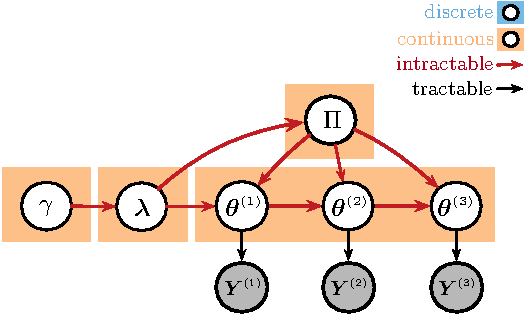
\includegraphics[width=0.49\linewidth]{../../fig/graphical_models/pgds.pdf}}\hfill
%
\subfigure[Poisson-randomized gamma dynamical systems]
{\label{fig:prgds}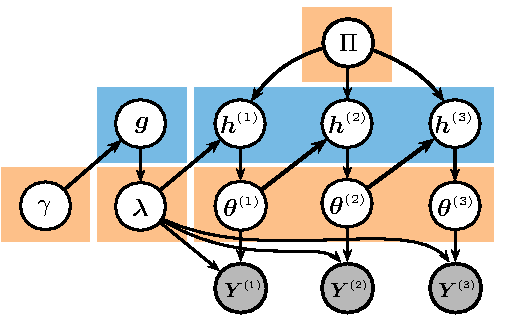
\includegraphics[width=0.49\linewidth]{../../fig/graphical_models/prgds.pdf}}
\caption{\label{fig:comparison} \footnotesize \emph{Left}: The PGDS imposes dependencies directly between the gamma latent states, preventing closed-form complete conditionals. \emph{Right}: The PrGDS (this paper) breaks these dependencies with discrete Poisson latent states---doing so yields closed-form conditionals for all variables without data augmentation.~\looseness=-1}%\vspace{-1.5em}
\end{figure*}

This paper fills a gap in the literature between Poisson factorization models that are tractable---i.e., yielding closed-form complete conditionals that make inference algorithms easy to derive---and those that are expressive---i.e., capable of capturing a variety of complex dependence structures. To do so, we introduce an alternating chain of discrete Poisson and continuous gamma latent states, a new modeling motif that is analytically convenient and computationally tractable. We rely on this motif to construct the Poisson-randomized gamma dynamical system (PrGDS), a model for sequentially observed count tensors that is tractable, expressive, and efficient. The PrGDS is closely related to the Poisson--gamma dynamical system (PGDS) \cite{schein2016poisson}, a recently introduced model for dynamic count matrices, that is based on non-conjugate chains of gamma states. These chains are intractable; thus, posterior inference in the PGDS relies on sophisticated data augmentation schemes that are cumbersome to derive and impose unnatural restrictions on the priors over other variables. In contrast, the PrGDS introduces intermediate Poisson states that break the intractable dependencies between the gamma states (see \cref{fig:comparison}). Although this motif is only semi-conjugate, it is tractable, yielding closed-form complete conditionals for the Poisson states by way of the little-known Bessel distribution~\cite{yuan2000bessel} and a novel discrete distribution that we derive and call the \emph{shifted confluent hypergeometric (SCH) distribution}.~\looseness=-1

We study the inductive bias of the PrGDS by comparing its smoothing and forecasting abilities to those of the PGDS and two other baselines on a range of real-world count data sets of text, international events, and neural spike data. We find that the PrGDS often obtains lower smoothing and forecasting perplexities than the PGDS and related baselines. Using a specific hyperparameter setting, the PrGDS permits the gamma states to take values of exactly zero, thereby encoding a unique inductive bias tailored to sparsity and burstiness. We find that this variant often obtains lower smoothing and forecasting perplexities than other models. We also find that this variant yields a qualitatively broader range of latent structures---specifically, bursty latent structures that are highly localized in time.~\looseness=-1

% We present the PrGDS in \cref{sec:prgds} and detail its connections to prior work in \cref{sec:bg}. In \cref{sec:mcmc}, we show that PrGDS admits closed-form complete conditionals for all variables without any data augmentation. To do so, in \cref{sec:recursion}, we discuss and derive identities about the general motif on which PrGDS is based. In \cref{sec:empirical}, we study the inductive bias of the PrGDS by comparing its smoothing and forecasting ability to the PGDS and two other baselines on a range of real-world count matrices and tensors of text, international events, and neural spike data. We find that the PrGDS often obtains lower smoothing and forecasting perplexity than the PrGDS and related baselines. The PrGDS under a specific hyperparameter settings permits the continuous states to take values of \emph{exactly} zero thus encoding a unique inductive bias tailored to sparsity and burstiness. We find that this variant, in particular, often obtains the lowest perplexity of all models and additionally infers qualitatively different latent structure that is highly localized in time.~\looseness=-1

% Beyond political science, sequentially observed count tensors are the object of analysis in many scientific disciplines. Neuroscientists, for instance, apply tensor decomposition methods to tensors of neuron spike counts to infer interpretable structure that can be explored to suggest new scientific theories about animal behavior and cognition \cite{williams2018unsupervised}.

% In addition to being uniquely capable of inferring highly localized latent structure,
% \pagebreak
\section{Poisson-randomized gamma dynamical systems (PrGDS)}
\label{sec:prgds}

\textbf{Notation.} Consider a data set of sequentially observed count tensors $\boldsymbol{Y}^{\mathsmaller{(1)}},\dots,\boldsymbol{Y}^{\mathsmaller{(T)}}$, each of which has $M$ modes. An entry $\ydt \!\in\! \{0,1,2,\dots\}$ in the $t^{\textrm{th}}$ tensor is subscripted by a multi-index $\osubs \equiv (\osub_1,\dots,\osub_M)$ that indexes into the $M$ modes of the tensor. As an example, the event count of the number of times country $i$ took action $a$ toward country $j$ during time step $t$ can be written as $\ydt$  where the multi-index corresponds to the sender, receiver, and action type---i.e., $\osubs = (i, j, a)$.~\looseness=-1

\textbf{Generative process.} The PrGDS is a form of canonical polyadic decomposition \cite{harshman1970foundations} that models $\yd$ as~\looseness=-1
\begin{align}
\label{eq:tensor_likelihood}
\ydt &\sim \textrm{Pois}\Big(\rhot \sum_{k = 1}^K \lambda_k \, \thetakt \prod_{m=1}^M \phi^{\mathsmaller{(m)}}_{k \osub_m}\Big),
\end{align}
where $\thetakt$ represents the activation of the $k^{\textrm{th}}$ component at time step $t$. Each component represents a dependence structure in the data set by way of a factor vector $\boldsymbol{\phi}^{\mathsmaller{(m)}}_{k}$ for each mode $m$. For international events, the first factor vector $\boldsymbol{\phi}^{\mathsmaller{(1)}}_{k} \teq (\phi^{\mathsmaller{(1)}}_{k1},\dots,\phi^{\mathsmaller{(1)}}_{kV})$ represents the rate at which each of the $V$ countries acts as a sender in the $k^{\textrm{th}}$ component while the second factor vector $\boldsymbol{\phi}^{\mathsmaller{(2)}}_{k}$ represents the rate at which each country acts as a receiver. The weights $\lambda_k$ and $\rho^{\mathsmaller{(t)}}$ represent the scales of component $k$ and time step $t$. The PrGDS is stationary if $\rhot \teq \rho$. We posit the following conjugate priors:~\looseness=-1
% there is a set of factors $\phi^{\mathsmaller{(m)}}_{k \osub_m}$ for each mode $m$ that represents the strength of feature $i_{m}$ in component $k$. An analogous generalization can be made of the PGDS. However, as before, the ``augment-and-conquer'' inference is only available if $\lambda_k=\lambda$ and $\sum_{i_m=1}^{L_m} \phi^{\mathsmaller{(m)}}_{k \osub_m} \teq 1$ for all $m$. A secondary contribution of this paper is the generalization of the PGDS to tensor-valued time series which we use in \cref{sec:empirical} as a baseline. We provide the relevant inference equations in the Appendix and will open source our Cython implementation.
\begin{equation}
\rhot \sim \Gam{a_0, b_0} \,\,\,\textrm{ and }\,\,\, \boldsymbol{\phi}^{\mathsmaller{(m)}}_k \sim \textrm{Dir}(a_0,\dots,a_0).
\end{equation}
The PrGDS is characterized by an alternating chain of discrete and continuous latent states. The continuous states $\theta^{\mathsmaller{(1)}}_k, \ldots, \theta^{\mathsmaller{(T)}}_k$ evolve via the intermediate discrete states $h^{\mathsmaller{(1)}}_k, \ldots, h^{\mathsmaller{(T)}}_k$ as follows:~\looseness=-1
\begin{equation}
\label{eq:thetaktandhkt}
\thetakt \sim \Gam{\epstheta \tp \hkt,\, \tau} \,\,\textrm{ and }\,\, \hkt \sim \textrm{Pois}\Big(\tau \sum_{k_2 = 1}^K \pi_{kk_2} \,\thetakttm\Big),
\end{equation}
where $\thetakt$ is the per-component weight from \cref{eq:tensor_likelihood} and $\theta^{\mathsmaller{(0)}}_k \teq \lambda_k$. In other words, the PrGDS assumes that $\thetakt$ is conditionally gamma distributed with rate $\tau$ and shape equal to $\hkt$ plus hyperparameter $\epstheta \geq 0$. We adopt the convention that a gamma random variable will be zero, almost surely, if its shape is zero. Therefore, setting $\epstheta \teq 0$ defines a sparse variant of the PrGDS, where the gamma latent state $\thetakt$ takes the value of exactly zero provided $\hkt \teq 0$---i.e., $\thetakt \stackrel{\textrm{a.s.}}{=} 0$ if $\hkt \teq 0$.~\looseness=-1

The \emph{transition weight} $\pi_{kk_2}$ in \cref{eq:thetaktandhkt} represents how strongly component $k_2$ excites component $k$ at the next time step. We view these weights collectively as a $K \!\times\! K$ transition matrix $\Pi$ and impose Dirichlet priors over the columns of this matrix. We also place a gamma prior over concentration parameter $\tau$. This prior is conjugate to the gamma and Poisson distributions in which it appears:~\looseness=-1
\begin{equation}
\tau \sim \Gam{\alpha_0, \alpha_0} \,\,\textrm{ and }\,\,
\boldsymbol{\pi}_k \sim \textrm{Dir}\left(a_0,\dots,a_0\right) \textrm{ such that }\mathsmaller{\sum_{k_1}}^K \pi_{k_1k}=1.
\end{equation}
% \begin{align}
% \mathbb{E}\left[\boldsymbol{\theta}^{\mathsmaller{(t)}} \given \boldsymbol{\theta}^{\mathsmaller{(t \tm 1)}}\right] = \mathbb{E}\left[\mathbb{E}\left[\boldsymbol{\theta}^{\mathsmaller{(t)}} \given \boldsymbol{h}^{\mathsmaller{(t \tm 1)}}\right]\right] = \Pi \, (\boldsymbol{\theta}^{\mathsmaller{(t \tm 1)}} \odot \boldsymbol{\eta})
% \end{align}
% When $\epstheta > 0$, this construction corresponds to the \emph{randomized gamma of the first type}~\citep{yuan2000bessel,makarov2010exact} while when $\epstheta=0$ this construction corresponds to the Poisson-randomized gamma distribution~\citep{zhou2016augmentable}.
% Thus, $\tau$ mainly controls the variance of the latent dynamics while only affecting the expectation by a factor of $\epstheta$ (and not at all when $\epstheta \teq 0$). We impose the  prior $\tau \sim \Gam{\alpha_0, \alpha_0}$ which is conjugate to both the Poisson and gamma distributions in which $\tau$ appears.
For the per-component weights $\lambda_1, \ldots, \lambda_K$, we use a hierarchical prior with a similar flavor to \cref{eq:thetaktandhkt}:~\looseness=-1
\begin{equation}
\label{eq:lambdakandgk}
\lambda_k \sim \textrm{Gam}\Big(\tfrac{\epslambda}{K} + g_k,\, \beta\Big) \,\,\textrm{ and }\,\,g_k \sim \Pois{\tfrac{\gamma}{K}},
%
\end{equation}
where $\epslambda$ is analogous to $\epstheta$. Finally, we use the following gamma priors, which are both conjugate:~\looseness=-1
\begin{equation}
\gamma \sim \Gam{a_0,b_0} \,\,\,\textrm{ and }\,\,\, \beta \sim \Gam{\alpha_0, \alpha_0}.
\end{equation}
The PrGDS has five fixed hyperparameters: $\epstheta$, $\epslambda$, $\alpha_0$, $a_0$, and $b_0$. For the empirical studies in \cref{sec:empirical}, we set $a_0\teq b_0 \teq 0.01$ to define weakly informative gamma and Dirichlet priors and set $\alpha_0 \teq 10$ to define a gamma prior that promotes values close to 1; we consider $\epstheta \in \{0,1\}$ and set $\epslambda \teq 1$.~\looseness=-1

\textbf{Properties.}
In \cref{eq:lambdakandgk}, both $\epslambda$ and $\gamma$ are divided by the number of components $K$. This means that as the number of components grows $K \!\rightarrow\! \infty$, the expected sum of the weights remains finite and fixed:~\looseness=-1
\begin{equation}
\sum_{k=1}^\infty \E{\lambda_k} = \sum_{k=1}^\infty \big(\tfrac{\epslambda}{K} + \E{g_k}\big) \beta^{-1} = \sum_{k=1}^\infty \big(\tfrac{\epslambda}{K} + \tfrac{\gamma}{K} \big)\beta^{-1} = \big(\epslambda + \gamma \big)\beta^{-1}.
\end{equation}
This prior encodes an inductive bias toward small values of $\lambda_k$ and may be interpreted as the finite truncation of a novel Bayesian nonparametric process. A small value of $\lambda_k$ shrinks the Poisson rates of both $\ydt$ and the first discrete latent state $h^{\mathsmaller{(0)}}_k$. As a result, this prior encourages the PrGDS to only infer components that are both predictive of the data and useful for capturing the temporal dynamics.~\looseness=-1

The marginal expectation of $\boldsymbol{\theta}^{\mathsmaller{(t)}} \teq (\theta^{\mathsmaller{(t)}}_{1},\ldots,\theta^{\mathsmaller{(t)}}_{K})$ takes the form of a linear dynamical system:~\looseness=-1
\begin{align}
\label{eq:expectation}
\mathbb{E}\left[\boldsymbol{\theta}^{\mathsmaller{(t)}} \given \boldsymbol{\theta}^{\mathsmaller{(t \tm 1)}}\right] = \mathbb{E}\left[\mathbb{E}\left[\boldsymbol{\theta}^{\mathsmaller{(t)}} \given \boldsymbol{h}^{\mathsmaller{(t \tm 1)}}\right]\right] = \epstheta \tau^{-1} + \Pi \, \boldsymbol{\theta}^{\mathsmaller{(t \tm 1)}}.
\end{align}
This is because $\E{\thetakt} \teq \big(\epstheta \tp \E{\hkt}\big)\tau^{-1} \teq \big(\epstheta \tp \tau \sum_{k_2 = 1}^K \pi_{kk_2} \,\thetakttm \big) \tau^{-1}$ by iterated expectation. Concentration parameter $\tau$ appears in both the Poisson and gamma distributions in \cref{eq:thetaktandhkt}. It contributes to the variance of the PrGDS, while simultaneously canceling out of the expectation in \cref{eq:expectation}, except for its role in the additive term $\epstheta \tau^{-1}$, which itself disappears when $\epstheta \teq 0$.~\looseness=-1

Finally, we can analytically marginalize out all of the discrete Poisson latent states to obtain a purely continuous linear dynamical system. When $\epstheta > 0$, this dynamical system can be written as follows:
\begin{equation}
\label{eq:rg1}
\
\thetakt \sim \textrm{RG1}\Big(\epstheta,\,\tau\sum_{k_2=1}^K \pi_{kk_2} \thetakttm,\, \tau\Big),
%
% \,\,\textrm{ such that }\,\, \mathbb{E}\left[\boldsymbol{\theta}^{\mathsmaller{(t)}} \given \boldsymbol{\theta}^{\mathsmaller{(t \tm 1)}}\right] = \tfrac{\epstheta}{\tau} + \Pi \, \boldsymbol{\theta}^{\mathsmaller{(t \tm 1)}}.
\end{equation}
where RG1 denotes the randomized gamma distribution of the first type \cite{yuan2000bessel,makarov2010exact}. When $\epstheta \teq 0$, the dynamical system can be written in terms of a limiting form of the RG1. We describe the RG1 in \cref{fig:rg1}.~\looseness=-1

% \pagebreak
\section{Related work}
\label{sec:bg}
\begin{figure}[t]
\centering
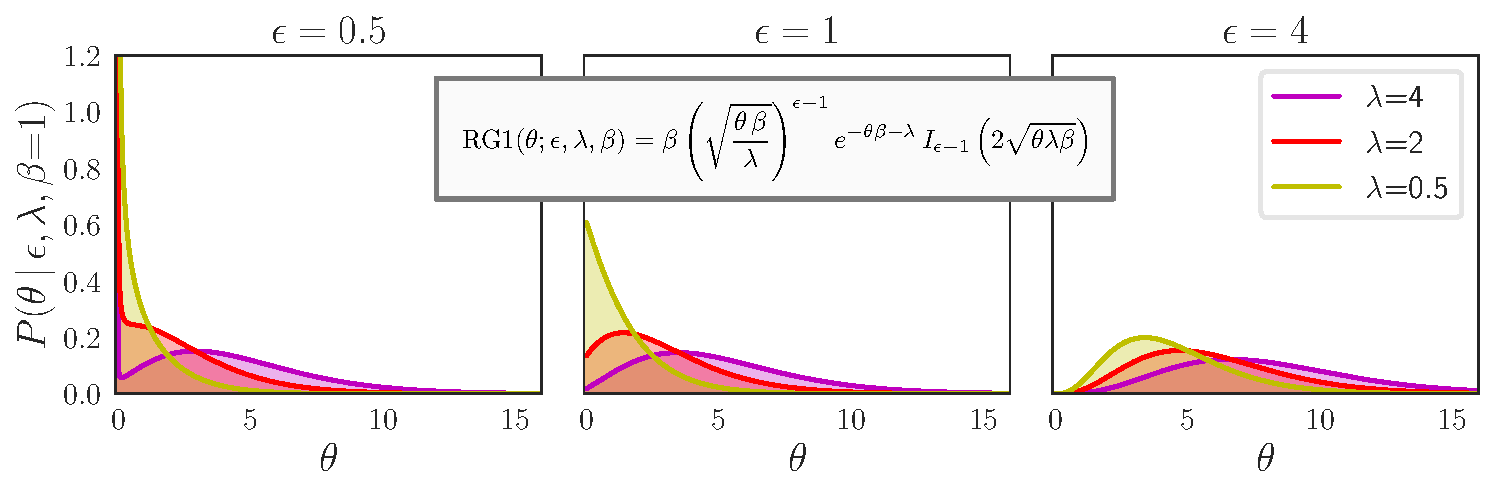
\includegraphics[width=\linewidth]{../../fig/distributions/annotated_rg1.pdf}
\caption{\footnotesize \label{fig:rg1} The randomized gamma distribution of the first type (RG1) \cite{yuan2000bessel,makarov2010exact} has support $\theta \!>\!  0$ and is defined by three parameters: $\epsilon$, $\lambda$, $\beta \!>\! 0$. Its PDF is displayed in the figure; $I_{\epsilon - 1}(\cdot)$ is the modified Bessel function of the first kind \cite{abramowitz1965handbook}. When $\epsilon < 1$ (\emph{left}), the RG1 resembles a soft ``spike-and-slab'' distribution; when $\epsilon \geq 1$ (\emph{middle and right}), it resembles a more-dispersed form of the gamma distribution. The Poisson-randomized gamma distribution \cite{zhou2016augmentable}, which includes zeros in its support (i.e., $\theta \geq 0$), is a limiting case of the RG1 that occurs when $\epsilon \!\rightarrow\! 0$.~\looseness=-1}%\vspace{-0.5em}
\end{figure}
The PrGDS is closely related to the Poisson--gamma dynamical system (PGDS)~\citep{schein2016poisson}. In the PGDS,~\looseness=-1%\vspace{-0.2em}
\begin{equation}
\label{eq:pgds}
\thetakt \sim \textrm{Gam}\Big(\tau\,\sum_{k_2=1}^K \pi_{kk_2} \thetakttm,\, \tau\Big)\,\,\textrm{ such that }\,\,
%
\mathbb{E}\left[\boldsymbol{\theta}^{\mathsmaller{(t)}} \given \boldsymbol{\theta}^{\mathsmaller{(t \tm 1)}}\right]= \Pi \, \boldsymbol{\theta}^{\mathsmaller{(t \tm 1)}}.
\end{equation}
The PGDS imposes non-conjugate dependencies directly between the gamma latent states. The complete conditional $P(\thetakt | -)$ is not available in closed form, and posterior inference relies on a sophisticated data augmentation scheme. The PrGDS instead introduces intermediate Poisson states that break the intractable dependencies between the gamma states; we visualize this in \cref{fig:comparison}. Although the Poisson distribution is not a conjugate prior for the gamma rate, this motif is still tractable, yielding the complete conditional $P(\hkt | -)$ in closed form, as we explain in \cref{sec:mcmc}. The PGDS is limited by the data augmentation scheme that it relies on for posterior inference---specifically, this augmentation scheme does not allow $\lambda_k$ to appear in the Poisson rate of $\ydt$ in \cref{eq:tensor_likelihood}. To encourage parsimony, the PGDS instead draws $\lambda_k \sim \textrm{Gam}(\tfrac{\gamma}{K}, \beta)$ and then uses these per-component weights to shrink the transition matrix $\Pi$. This approach introduces additional intractable dependencies that require a different data augmentation scheme for posterior inference. Finally, the data augmentation schemes additionally require that each factor vector $\boldsymbol{\phi}_k^{\mathsmaller{(m)}}$ and each column $\boldsymbol{\pi}_k$ of the transition matrix are Dirichlet distributed. We note that although we also use Dirichlet distributions in this paper, this is a choice rather than a requirement imposed by the PrGDS.~\looseness=-1

The PGDS and its ``deep'' variants~\cite{gong2017deep,guo2018deep} generalize gamma process dynamic Poisson factor analysis (GP-DPFA)~\citep{acharya2015nonparametric}, which assumes a simple random walk $\thetakt \tsim \Gam{\theta^{\mathsmaller{(t \tm 1)}}_k,\, c^{\mathsmaller{(t)}}}$; the model of Yang and Koeppl is also closely related~\cite{yang2018dependent}. These models belong to a line of work exploring the ``augment-and-conquer'' data augmentation scheme~\cite{zhou2012augment-and-conquer} for posterior inference in hierarchies of gamma variables chained via their shapes and linked to Poisson observations. Beyond models for time series, this motif can be used to build belief networks~\cite{zhou2015poisson}. An alternative approach is to chain gamma variables via their rates---e.g., $\theta^{\mathsmaller{(t)}} \sim \Gam{a,\,\theta^{\mathsmaller{(t\tm 1)}}}$. This motif is conjugate and tractable, and has been applied to models for time series~\cite{cemgil2007conjugate,fevotte2013non,jerfel2016dynamic} and deep belief networks~\cite{ranganath2015deep}. However, unlike the shape, the rate contributes to the variance of the gamma quadratically. Rate chains can therefore be highly volatile.~\looseness=-1

More broadly, gamma shape and rate chains are examples of non-negative chains. Such chains are especially well motivated in the context of Poisson factorization, which is particularly efficient when only non-negative prior distributions are used. In general, Poisson factorization assumes that each observed count $\yd$ is drawn from a Poisson distribution with a latent rate $\mud$ that is some function of the model parameters---i.e., $\yd \sim \Pois{\mud}$. When the rate is linear---i.e., $\mud \teq \sum_{k=1}^K \mu_{\osubs k}$---Poisson factorization is allocative~\citep{schein2019allocative} and admits a latent source representation~\cite{Dunson2005bayesianlatent,cemgil2009bayesian}, where $\yd \triangleq \sum_{k=1}^K y_{\osubs k}$ is defined to be the sum of $K$ latent sources $y_{\osubs 1}, \ldots, y_{\osubs K}$ and $y_{\osubs k} \sim \Pois{\mu_{\osubs k}}$. Conditioning on the latent sources often induces conditional independencies that, in turn, facilitate closed-form, efficient, and parallelizable posterior inference. The first step in either MCMC or variational inference is therefore to update each latent source from its complete conditional, which is multinomial \cite{steel1953relation}:~\looseness=-1
\begin{equation}
\label{eq:thinning}
\compcond{(y_{\osubs1},\dots,y_{\osubs K})} \sim \Multi{\yd,\, (\mu_{\osubs 1},\dots, \mu_{\osubs K})},
\end{equation}
where the normalization of the non-negative rates $\mu_{\osubs 1}, \ldots, \mu_{\osubs K}$ into a probability vector is left implicit. When the observed count is zero---i.e., $\yd \teq 0$---the sources are also zero---i.e., $y_{\osubs k} \stackrel{\textrm{a.s.}}{=}0$---and no computation is required to update them. As a result, any Poisson factorization model that admits a latent source representation scales linearly with only the non-zero entries. This property is indispensable when modeling count tensors which typically contain exponentially more zeros than non-zeros~\cite{bhattacharya2012simplex}. We emphasize that although the PrGDS and PGDS are substantively different models, they are both instances of allocative Poisson factorization, so the time complexity of posterior inference for both models is the same and equal to $\mathcal{O}\left(SK\right)$ where $S$ is the number of non-zero entries.~\looseness=-1

Because a latent source representation is only available when the rate $\mud$ is a linear function of the model parameters and, by definition of the Poisson distribution, the rate must be non-negative, efficient Poisson factorization is only possible with non-negative priors. Modeling time series and other complex dependence structures via efficient Poisson factorization therefore requires developing novel motifs that exclude the Gaussian priors that researchers have traditionally relied on for analytic convenience and tractability. For example, the Poisson linear dynamical system~\cite{smith2003estimating, paninski2010new, macke2011empirical} links the widely used Gaussian linear dynamical system~\cite{kalman1961new,ghahramani1999learning} to Poisson observations via an exponential link function---i.e., $\mud = \exp\left({\sum_k \cdots}\right)$. This approach, which is based on the generalized linear model \cite{nelder1972generalized}, relies on a non-linear link function and therefore does not admit a latent source representation. Another approach is to use log-normal priors, as in dynamic Poisson factorization \cite{charlin2015dynamic}; however, the log-normal is not conjugate to the Poisson and therefore does not yield closed-form conditionals.

There is also a long tradition of autoregressive models for time series of counts, including variational autoregressive models~\cite{brandt2012bayesian} and models that are based on the Hawkes process \cite{hawkes1971spectra,blundell2012modelling,simma2012modeling,linderman2014discovering}. This approach avoids the challenge of constructing tractable state-space models from non-negative priors by modeling temporal correlations directly between the observed counts. However, for high-dimensional data, such as sequentially observed count tensors, an autoregressive approach is often impractical.~\looseness=-1

% As efficient Poisson factorization is  renewed interest \cite{cemgil2019bayesian}, the

% The PGDS is thus incompatible with gamma priors over the factors $\phi_{kv}$ which are widely used in practice \cite{cemgil2009bayesian,gopalan2015scalable,schein2015bayesian}. It is also incompatible with per-component weights $\lambda_k$ that are widely used in conjunction with Bayesian nonparametric shrinkage priors for implicit model selection \cite{acharya2015nonparametric,schein2016bayesian}.

% The concentration parameter $\tau$ in the PGDS is analogous to $\tau$ in the PrGDS in that it affects the variance of the latent dynamics without affecting the expected value. However, unlike in the PrGDS, it is treated as a fixed hyperparameter in the PGDS, since no natural conjugate prior exists when it appears in both the shape and rate of the gamma distribution.



% \section{Background}
% \label{sec:bg}



% The challenge we embrace in this paper is thus to construct expressive and structured priors from only non-negative distributions. A reasonable approach is to use the log-normal as a prior, as in Dynamic Poisson factorization~\cite{charlin2015dynamic}. A more natural approach is to use gamma and Dirichlet priors, which are conjugate to the Poisson distribution and yield analytically closed-form complete conditionals.

% We take a new approach in this paper. Instead of chaining gamma random variables directly, we introduce alternating chains of conditionally gamma- and Poisson- distributed states. This construction is \emph{semi}-conjugate yet yields closed-form complete conditionals for all states, as we show in \cref{sec:mcmc}.\looseness=-1



% Allocative Poisson matrix factorization \cite{canny2004gap,Dunson2005bayesianlatent,titsias2008infinite,cemgil2009bayesian,zhou2011beta,gopalan2013efficient,paisley2014bayesian}.

% Non-negative tensor decomposition \citep{cichocki2007non,kolda2009tensor} and probabilistic Poisson tensor decomposition \cite{chi2012tensors}, and Bayesian variants \cite{ermis2014bayesian,schein2015bayesian,schein2016bayesian}.

% See \cite{cemgil2019bayesian} for a review of this area along with connections.

% This family of models is underdeveloped due to the lack of tractable and convenient modeling motifs using only non-negative priors. We introduce a fundamentally novel motif and build a dynamical system with it that uses it to chain together dynamic latent states and uses it to shrink.


% Models that are not tailored to count data fail to make this distinction and thus tend to waste computation and statistical power on the exponentially-large number of zeros, as if each were as informative as a non-zero observation.


\section{Posterior inference}
\label{sec:mcmc}
Iteratively re-sampling each latent variable in the PrGDS from its complete conditional constitutes a Gibbs sampling algorithm. The complete conditionals for all variables are immediately available in closed form without data augmentation. We provide conditionals for the variables with non-standard priors below; the remaining conditionals are in the supplementary material. The PrGDS is based on a new motif in Bayesian latent variable modeling. We introduce the motif in its general form, derive its conditionals, and then use these to obtain the closed-form complete conditionals for the PrGDS.~\looseness=-1

\subsection{Poisson--gamma--Poisson chains}
\label{sec:recursion}
Consider the following model of count $m$ involving variables $\theta$ and $h$ and fixed $c_1, c_2, c_3, \epstheta >0$:
\begin{equation}
m \sim \Pois{\theta c_3},\,\,
%
\theta \sim \Gam{\epstheta \tp h, c_2},\,\,
%
\textrm{and}\,\, h \sim \Pois{c_1}.
\end{equation}
This model is semi-conjugate. The gamma prior over $\theta$ is conjugate to the Poisson and its posterior is
%
\begin{align}
\label{eq:gamma}
\compcond{\theta} &\sim \Gam{\epstheta \tp h + m,\, c_2 + c_3}.
\end{align}
The Poisson prior over $h$ is not conjugate to the gamma; however, despite this, the posterior of $h$ is still available in closed form by way of the Bessel distribution \cite{yuan2000bessel}, which we define in \cref{fig:bessel}:\looseness=-1
\begin{align}
\label{eq:bessel}
\compcond{h} &\sim \textrm{Bes}\big(\epstheta \tm 1,\, 2\sqrt{\theta \,c_2\, c_1}\big).
\end{align}
The Bessel distribution can be sampled efficiently \cite{devroye2002simulating}; our Cython implementation is available online.\footnote{\url{TODO}}
Provided that $\epstheta \!>\! 0$, sampling $\theta$ and $h$ iteratively from \cref{eq:gamma,eq:bessel} constitutes a valid Markov chain for posterior inference. When $\epstheta \teq 0$, though, $\theta \stackrel{\textrm{a.s.}}{=} 0$ if $h \teq 0$, and vice versa. As a result, this Markov chain has an absorbing condition at $h \teq 0$ and violates detailed balance. In this case, we must therefore sample $h$ with $\theta$ marginalized out. Toward that end, we prove Theorem 1.~\looseness=-1

\textbf{Theorem 1:} \textit{The incomplete conditional $P(h\given{\epstheta \teq 0, -\backslash} \theta)\triangleq \int P(h,\theta\given \epstheta \teq 0, -)\,\mathbf{d}\theta$ is}~\looseness=-1
\begin{align}
\label{eq:sch}
\left(h \given {-\backslash} \theta\right) &\sim
\begin{cases}
\textrm{Pois}\big(\frac{c_1\,c_2}{c_3+c_2}\big) &\textrm{if }m=0\\
\textrm{SCH}\big(m,\, \frac{c_1\,c_2}{c_3+c_2}\big)\, &\textrm{otherwise,}
\end{cases}
\end{align}
\textit{where SCH denotes the shifted confluent hypergeometric distribution. We describe the SCH in \cref{fig:sch} and provide further information in the supplementary material, including the derivation of its PMF, PGF, and mode, along with details of how we sample from it and the proof for Theorem 1.}~\looseness=-1

\begin{figure*}[t]
\centering
\subfigure[\footnotesize Bessel distribution~\cite{yuan2000bessel}]
{\label{fig:bessel}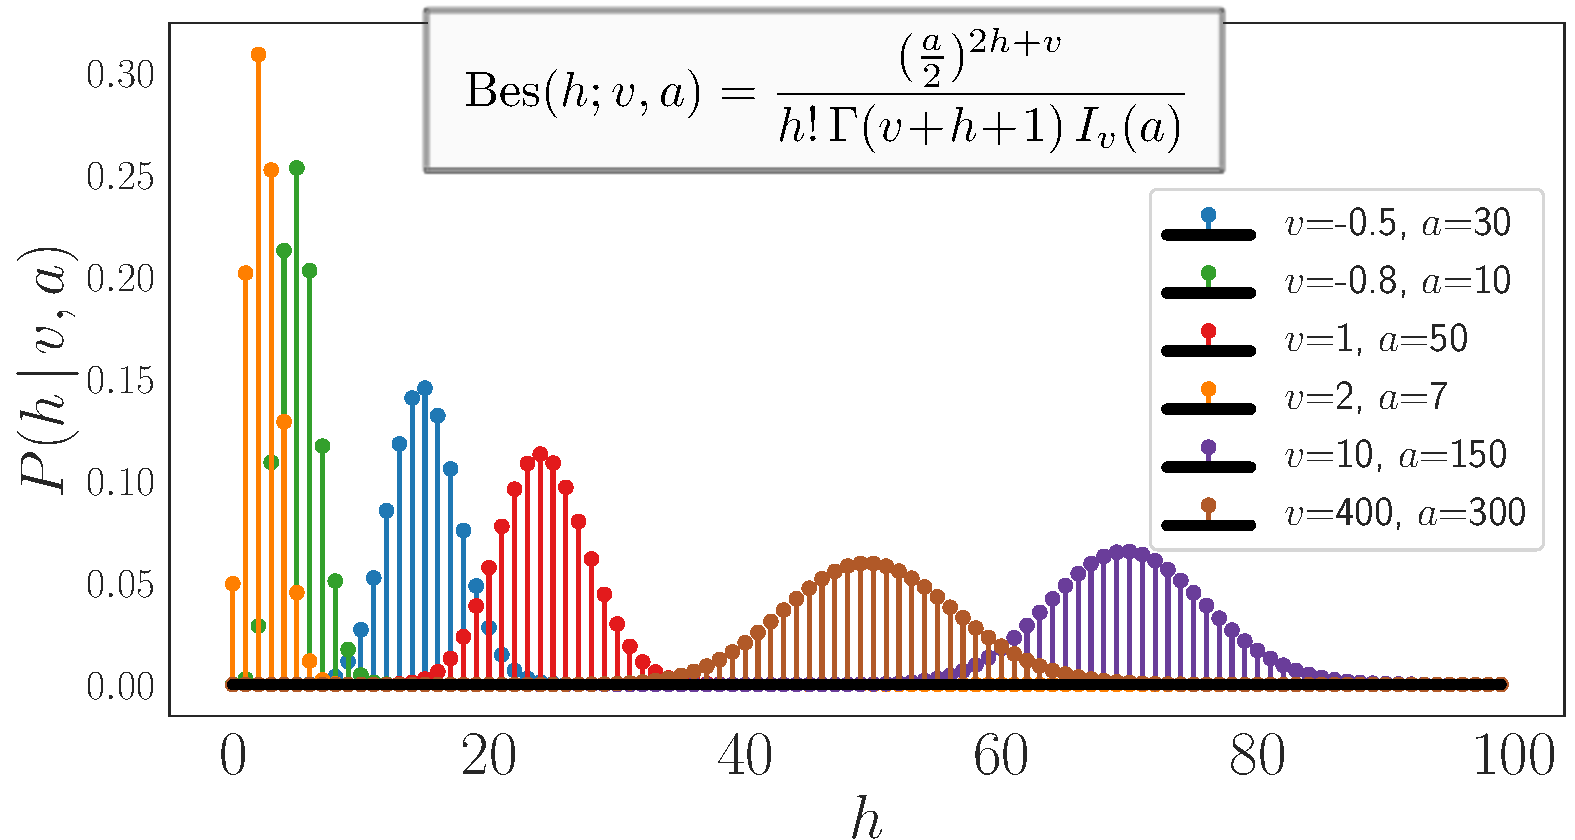
\includegraphics[width=0.5\linewidth]{../../fig/distributions/annotated_bessel.pdf}}\hfill
%
% \hspace{0.5em}
\subfigure[\footnotesize Shifted confluent hypergeometric (SCH) distribution]
{\label{fig:sch}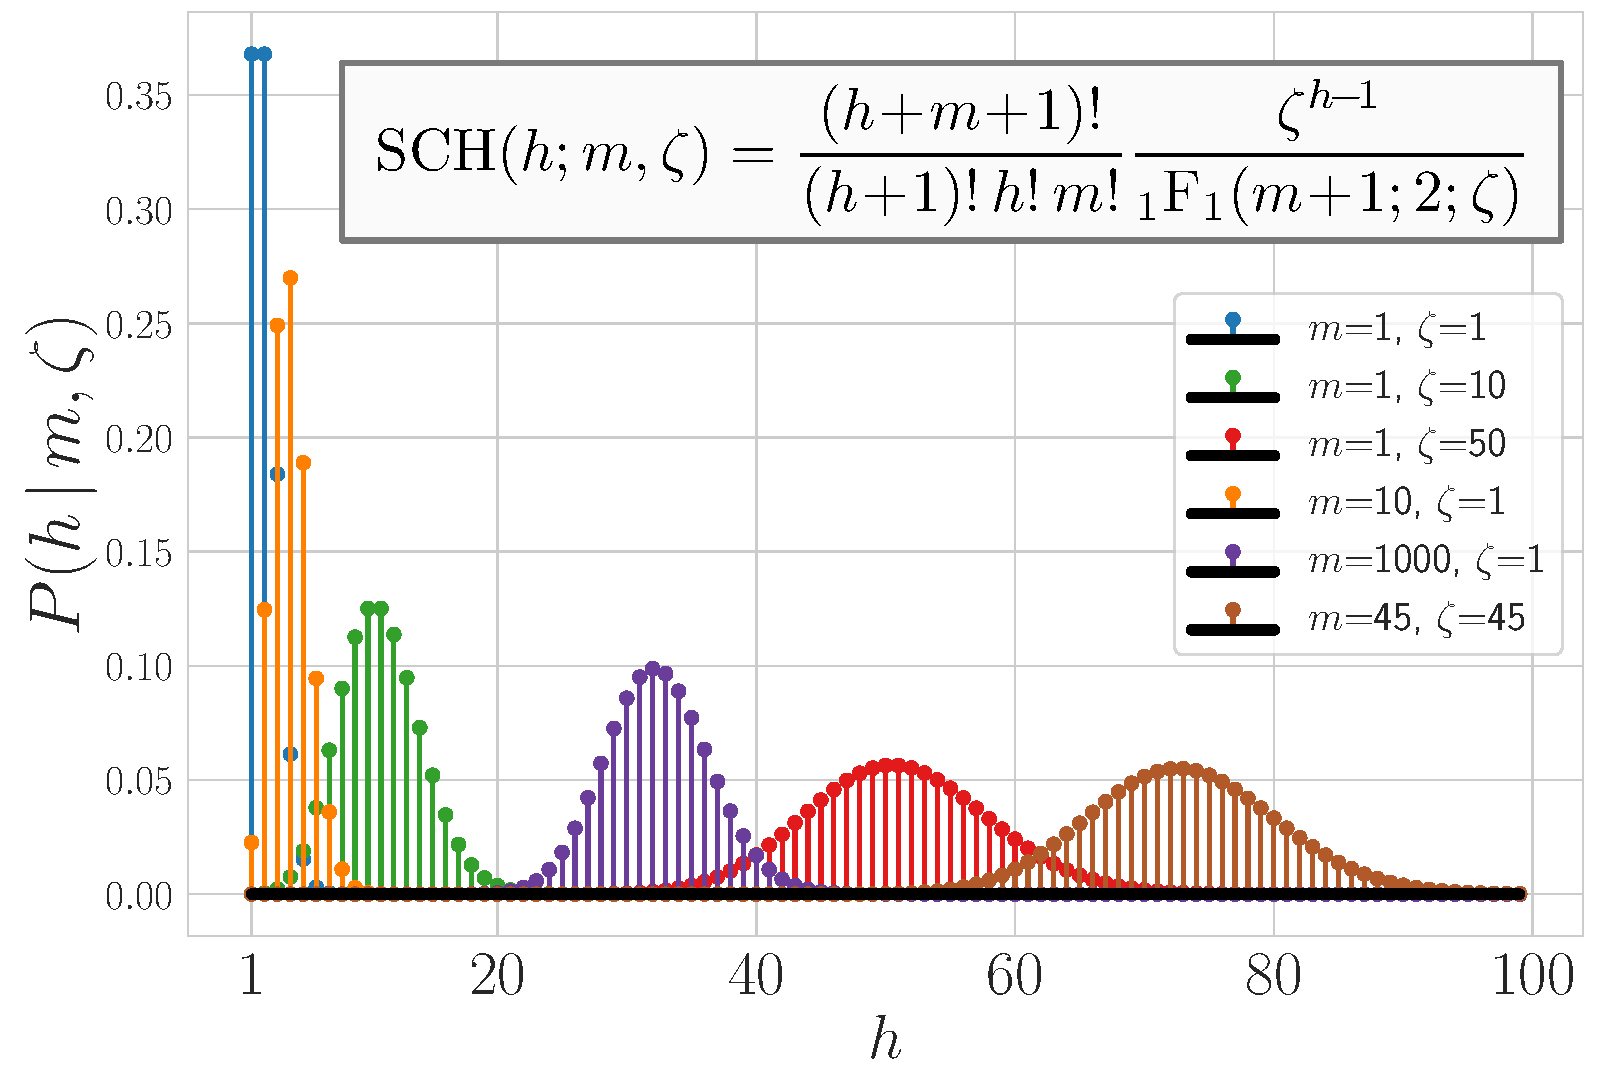
\includegraphics[width=0.5\linewidth]{../../fig/distributions/annotated_sch.pdf}}%\vspace{-0.5em}
\caption{\footnotesize \label{fig:distributions} Two discrete distributions that arise as posteriors in Poisson--gamma--Poisson chains.~\looseness=-1}%\vspace{-1em}
\end{figure*}

\subsection{Closed-form complete conditionals for the PrGDS}
The PrGDS admits a latent source representation, so the first step of posterior inference is therefore
\begin{align}
  \compcond{(y^{\mathsmaller{(t)}}_{\osubs k})_{k=1}^K} &\sim \Multi{\ydt,\big(\lambda_k \, \thetakt \mathsmaller{\prod}_{m=1}^M \phimki\big)_{k=1}^K}.
  \end{align}
We may similarly represent $\hkt$ as its latent source representation---i.e., $\hkt \tequiv \hkdt \teq \sum_{k_2=1}^K \hkkt$, where $\hkkt \tsim \Pois{\tau \, \pi_{kk_2} \thetakttm}$. When notationally convenient, we use dot-notation (``$\bcdot$'') to denote summing over an mode. In this case, $\hkdt$ denotes the sum of the $k^{\textrm{th}}$ row of the $K \ttimes K$ matrix of latent counts $\hkkt$. The complete conditional of the $k^{\textrm{th}}$ row of counts, when conditioned on their sum $\hkdt$, is~\looseness=-1
\begin{align}
\compcond{(\hkkt)_{k_2=1}^K} &\sim \Multi{\hkdt,\,(\pi_{kk_2} \thetakttm)_{k_2=1}^K}.
\end{align}
To derive the conditional for $\thetakt$ we aggregate the Poisson variables that depend on it. By Poisson additivity, the column sum $\hdktp \teq \sum_{k_1=1}^K h_{k_1k}^{\mathsmaller{(t \tp 1)}}$ is distributed as $\hdktp \tsim \Pois{\thetakt \, \tau\,\pi_{\bcdot k}}$ and similarly $y_{\bcdot k}^{\mathsmaller{(t)}}$ is distributed as $y_{\bcdot k}^{\mathsmaller{(t)}} \tsim \textrm{Pois}\big(\thetakt \rhot \lambda_k \prod_{m=1}^M\phi^{\mathsmaller{(m)}}_{k\bcdot}\big)$. The count $\mkt \triangleq \hdktp \tp \ykt$ isolates all dependence on $\thetakt$ and is also Poisson distributed. By gamma--Poisson conjugacy, the conditional of $\thetakt$ is~\looseness=-1
\begin{align}
% \footnote{We provide general equations but note they simplify with Dirichlet priors since $\pi_{\bcdot k} \teq 1$ and $\phi^{\mathsmaller{(m)}}_{\cdot k} \teq 1$.~\looseness=-1}
 %
  \compcond{\thetakt} &\sim \textrm{Gam}\big(\epstheta \tp \hkdt + \mkt,\, \tau + \tau\,\pi_{\bcdot k}+ \rhot \lambda_k \, \mathsmaller{\prod}_{m=1}^M \phi^{\mathsmaller{(m)}}_{k\bcdot }\big).
\end{align}
When $\epstheta > 0$, we apply the identity in \cref{eq:bessel} and sample $\hkdt$ from its complete conditional:
\begin{align}
\compcond{\hkdt} &\sim \textrm{Bessel}\Big(\epstheta \tm 1,\, 2 \sqrt{\thetakt \, \tau^2 \mathsmaller{\sum}_{k_2=1}^K \pi_{kk_2} \thetakttm}\Big).
\end{align}
When $\epstheta \teq0$, we instead apply Theorem 1 to sample $\hkdt$, where $\mkt$ is analogous to $m$ in \cref{eq:sch}:
%
\begin{align}
\left(\hkdt \given {-\backslash} \thetakt\right) &\sim
\begin{cases}
\textrm{Pois}(\zeta_{k}^{\mathsmaller{(t)}}) &\textrm{if } \mkt \teq 0 \\
%
\textrm{SCH}(\mkt,\, \zeta_{k}^{\mathsmaller{(t)}}) &\textrm{otherwise}
\end{cases}
\hspace{1em}\textrm{where }\,\,
\zeta_{k}^{\mathsmaller{(t)}} \triangleq \mathsmaller{\frac{\tau^2 \sum_{k_2=1}^K \pi_{kk_2} \thetakttm}{\tau + \tau\,\pi_{\bcdot k} + \rhot \lambda_k \prod_{m=1}^M\phi^{\mathsmaller{(m)}}_{k\bcdot }}}.
\end{align}
The complete conditionals for $\lambda_k$ and $g_k$ follow from applying the same Poisson--gamma--Poisson identities, while the complete conditionals for $\gamma$, $\beta$, $\boldsymbol{\phi}^{\mathsmaller{(m)}}_k$, $\boldsymbol{\pi}_{k}$, and $\tau$ all follow from conjugacy.% We provide them all in the Appendix.~\looseness=-1
% b

\section{Empirical studies}
\label{sec:empirical}
\begin{figure*}[t]
\centering
\subfigure[\footnotesize Matrix empirical studies (originally described by~\citet{schein2016poisson})]
{\label{fig:matrix_results}\includegraphics[width=0.669\linewidth]{../../results/matrices/test_new_matrix_results.pdf}}\hfill
%
\subfigure[Tensor empirical studies]
{\label{fig:tensor_results}\includegraphics[width=0.32\linewidth]{../../results/tensors/test_tensor_results.pdf}}%\vspace{-0.5em}
\caption{\label{fig:empirical}\footnotesize The smoothing (top row) or forecasting (bottom row) performance of each model is quantified by its log-perplexity---where lower values are better---divided by the log-perplexity of a non-dynamic baseline \cite{schein2015bayesian}.~\looseness=-1}%\vspace{-2em}
\end{figure*}

As explained in the previous section, the Poisson--gamma--Poisson motif of the PrGDS (see \cref{sec:recursion}) yields a more tractable (see \cref{fig:comparison}) and flexible (see \cref{sec:bg}) model than previous models. This motif also encodes a unique inductive bias tailored to sparsity and burstiness that we test by comparing the PrGDS to the PGDS (described in \cref{sec:bg}). As we can see by comparing \cref{eq:rg1,eq:pgds}, comparing these models isolates the impact of the Poisson--gamma--Poisson motif. Because the PGDS was previously introduced to model a $T \ttimes V$ matrix $Y$ of sequentially observed $V$-dimensional count vectors $\boldsymbol{y}^{\mathsmaller{(1)}},\dots, \boldsymbol{y}^{\mathsmaller{(T)}}$, we generalize the PGDS to $M$-mode tensors and provide derivations of its complete conditionals in the supplementary material. Our Cython implementation of this generalized PGDS (and the PrGDS) is available online. We also compare the variant of the PrGDS with $\epstheta \teq 1$~to~the variant with $\epstheta \teq 0$, which allows the gamma latent states to take values of exactly zero.\looseness=-1

\textbf{Setup.} Our empirical studies all have the following setup. For each data set $\Yten^{\mathsmaller{(1)}},\dots,\Yten^{\mathsmaller{(T)}}$, the counts $\Yten^{\mathsmaller{(t)}}$ in randomly selected time steps are held out. Additionally, the counts in the last two time steps are always held out. Each model is fit to the data set using independent MCMC chains that impute the heldout counts and, ultimately, return $S$ posterior samples of the latent variables. The posterior samples are then used to compute the expectation $\mudt$ of each heldout count $\ydt$ (as defined in \cref{eq:tensor_likelihood}). We distinguish the task of predicting the counts in intermediate time steps, known as smoothing, from the task of predicting the counts in the last two time steps, known as forecasting.
%
To quantify the performance of each model, we compute its log-perplexity---i.e., $\log \textrm{Perp}(\Delta) = -\frac{1}{|\Delta|}\sum_{(t,\osubs) \in \Delta} \log \Big[\frac{1}{S}\sum_{s=1}^S \textrm{Pois}\big(\ydt; \musdt \big) \Big]$, where $\Delta$ is the set of multi-indices of the heldout data and $\musdt$ is the expectation of heldout count $\ydt$ computed from the $s^{\textrm{th}}$ posterior sample.
%
Perplexity is a standard evaluation metric~\citep{wallach2009evaluation} that is inversely proportional to pointwise predictive density~\citep{gelman2014understanding}.
%
In each study, we fit a simple non-dynamic baseline---Bayesian Poisson tensor factorization (BPTF) \cite{schein2015bayesian}---and use it to predict the heldout counts. This model assumes that the count tensors at different time steps are i.i.d.---i.e., $y_{\osubs}^{\mathsmaller{(t)}} \tsim \Pois{\mud}$. We report the improvement of each of the dynamic models over BPTF by reporting its log-perplexity divided by the log-perplexity of BPTF.\looseness=-1

\textbf{Matrices.} We first replicated the empirical studies of~\citet{schein2016poisson}. These studies followed the setup described above and compared the PGDS to GP-DPFA \cite{acharya2015nonparametric}, a simple dynamic baseline (described in \cref{sec:bg}). The matrices in these studies were based on three text data sets---NeurIPS papers~\cite{neuripscorpus}, DBLP abstracts~\cite{dblp}, and State of the Union (SOTU) speeches~\cite{sotu}---where $\yvt$ is the number of times word $v$ occurs in time step $t$, and two international event data sets---GDELT \cite{leetaru2013gdelt} and ICEWS \cite{boscheeicews}---where $\yvt$ is the number of times sender--receiver pair $v$ interacted during time step $t$. We obtained the matrices and heldout time steps, along with the original results for both PGDS and GP-DPFA, from the authors. We fit the PrGDS with the MCMC settings that they describe (see their paper  \cite{schein2016poisson} for details) and fit BPTF using variational inference. We depict the results in \cref{fig:matrix_results}.~\looseness=-1

\textbf{Tensors.} We used two international event data sets---GDELT and ICEWS---where $y_{\mathsmaller{i \xrightarrow{a}j}}^{\mathsmaller{(t)}}$ is the number of times country $i$ took action $a$ toward country $j$ during time step $t$.
Each data set consists of a sequence of count tensors, each of which contains the $249 \ttimes 249 \ttimes 20$ event counts for that time step. For both data sets, we used months as time steps. For GDELT, we considered the date range 2003--2008 (i.e., $T \teq 72$); for ICEWS, we considered the date range 1995--2013 (i.e., $T \teq 228$). We also used multi-neuronal spike train recordings of macaque monkey motor cortexes collected and studied by~\citet{vyas2018neural} and~\citet{williams2018unsupervised}.  In this data set, a count $y^{\mathsmaller{(t)}}_{ij}$ is the number of times neuron $i$ spiked in trial $j$ during time step $t$. These counts form a sequence of $N \ttimes S$ matrices, where $N \teq 100$ is the number of neurons and $S \teq 1,716$ is the number of trials. We used 20-millisecond intervals as time steps, yielding $T \teq 162$. For each data set, we randomly selected six heldout time steps in the range $[2, T\tm 2]$. We fit each model using 4,000 MCMC iterations, saving every $100^{\textrm{th}}$ posterior sample after the first 1,000 iterations to compute its log-perplexity. We also fit BPTF using variational inference.~Following~\citet{schein2016poisson}, we set $K \teq 100$ for all models. We depict the results in \cref{fig:tensor_results}.\looseness=-1



% To measure predictive performance, we compute perplexity~\citep{wallach2009evaluation}, a standard evaluation metric that is inversely proportional to pointwise predictive density~\citep{gelman2014understanding}.


\begin{figure*}[t]
\centering
\subfigure[\footnotesize International event data]
{
\label{fig:sudan}
% 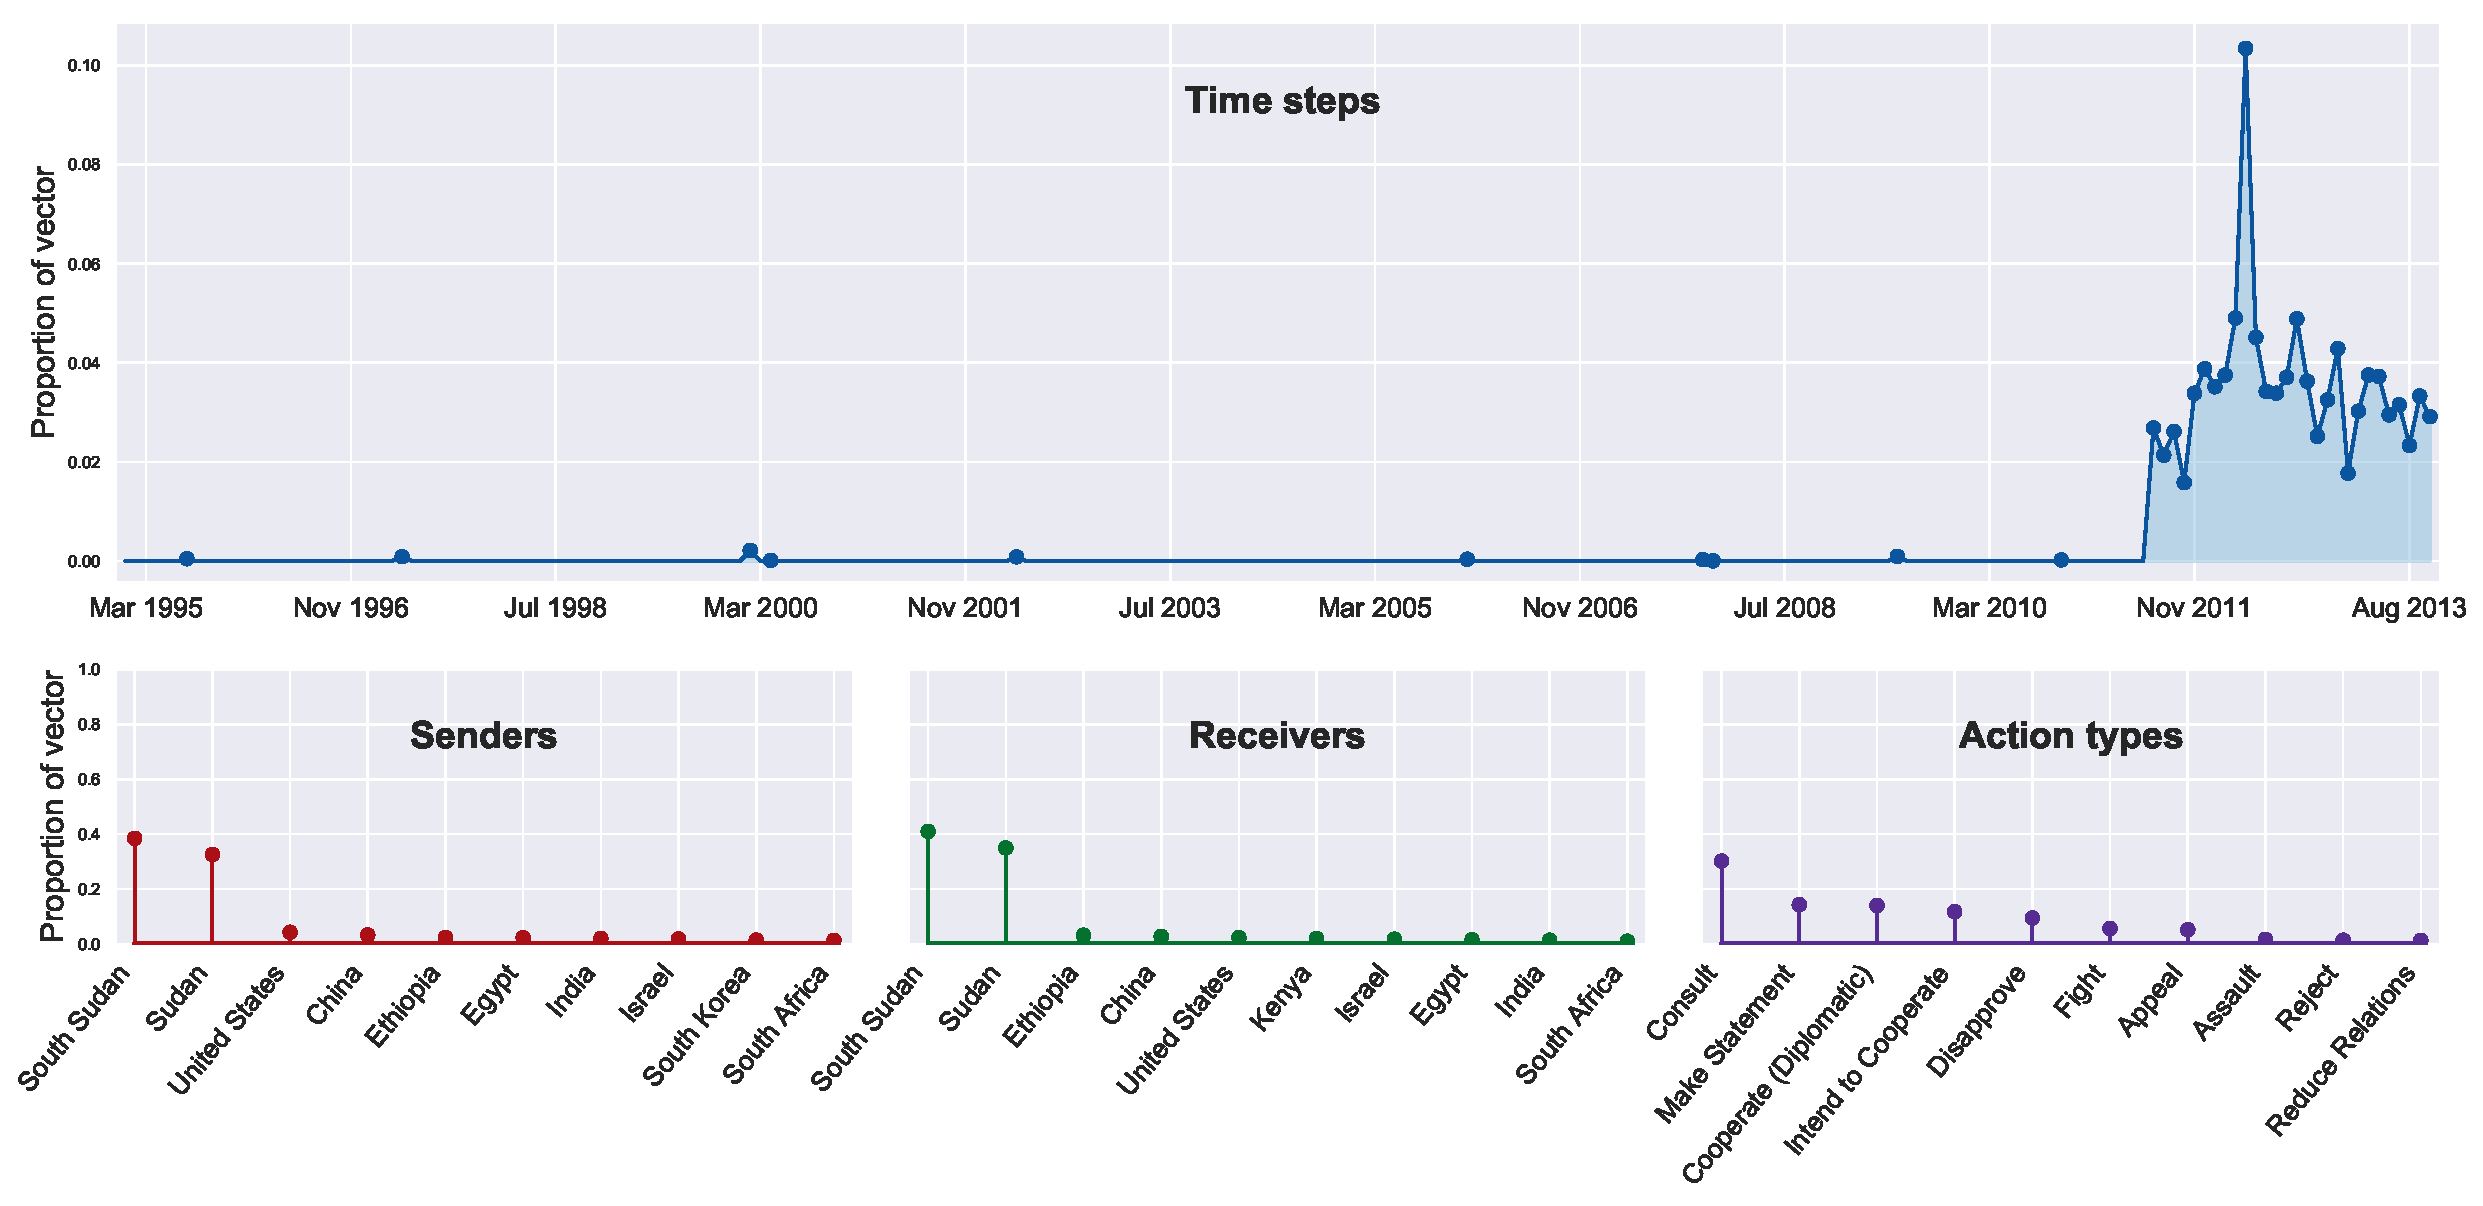
\includegraphics[width=\linewidth]{../../fig/components/icews/zero-ordering/new_plots/eps0-component-0.pdf}
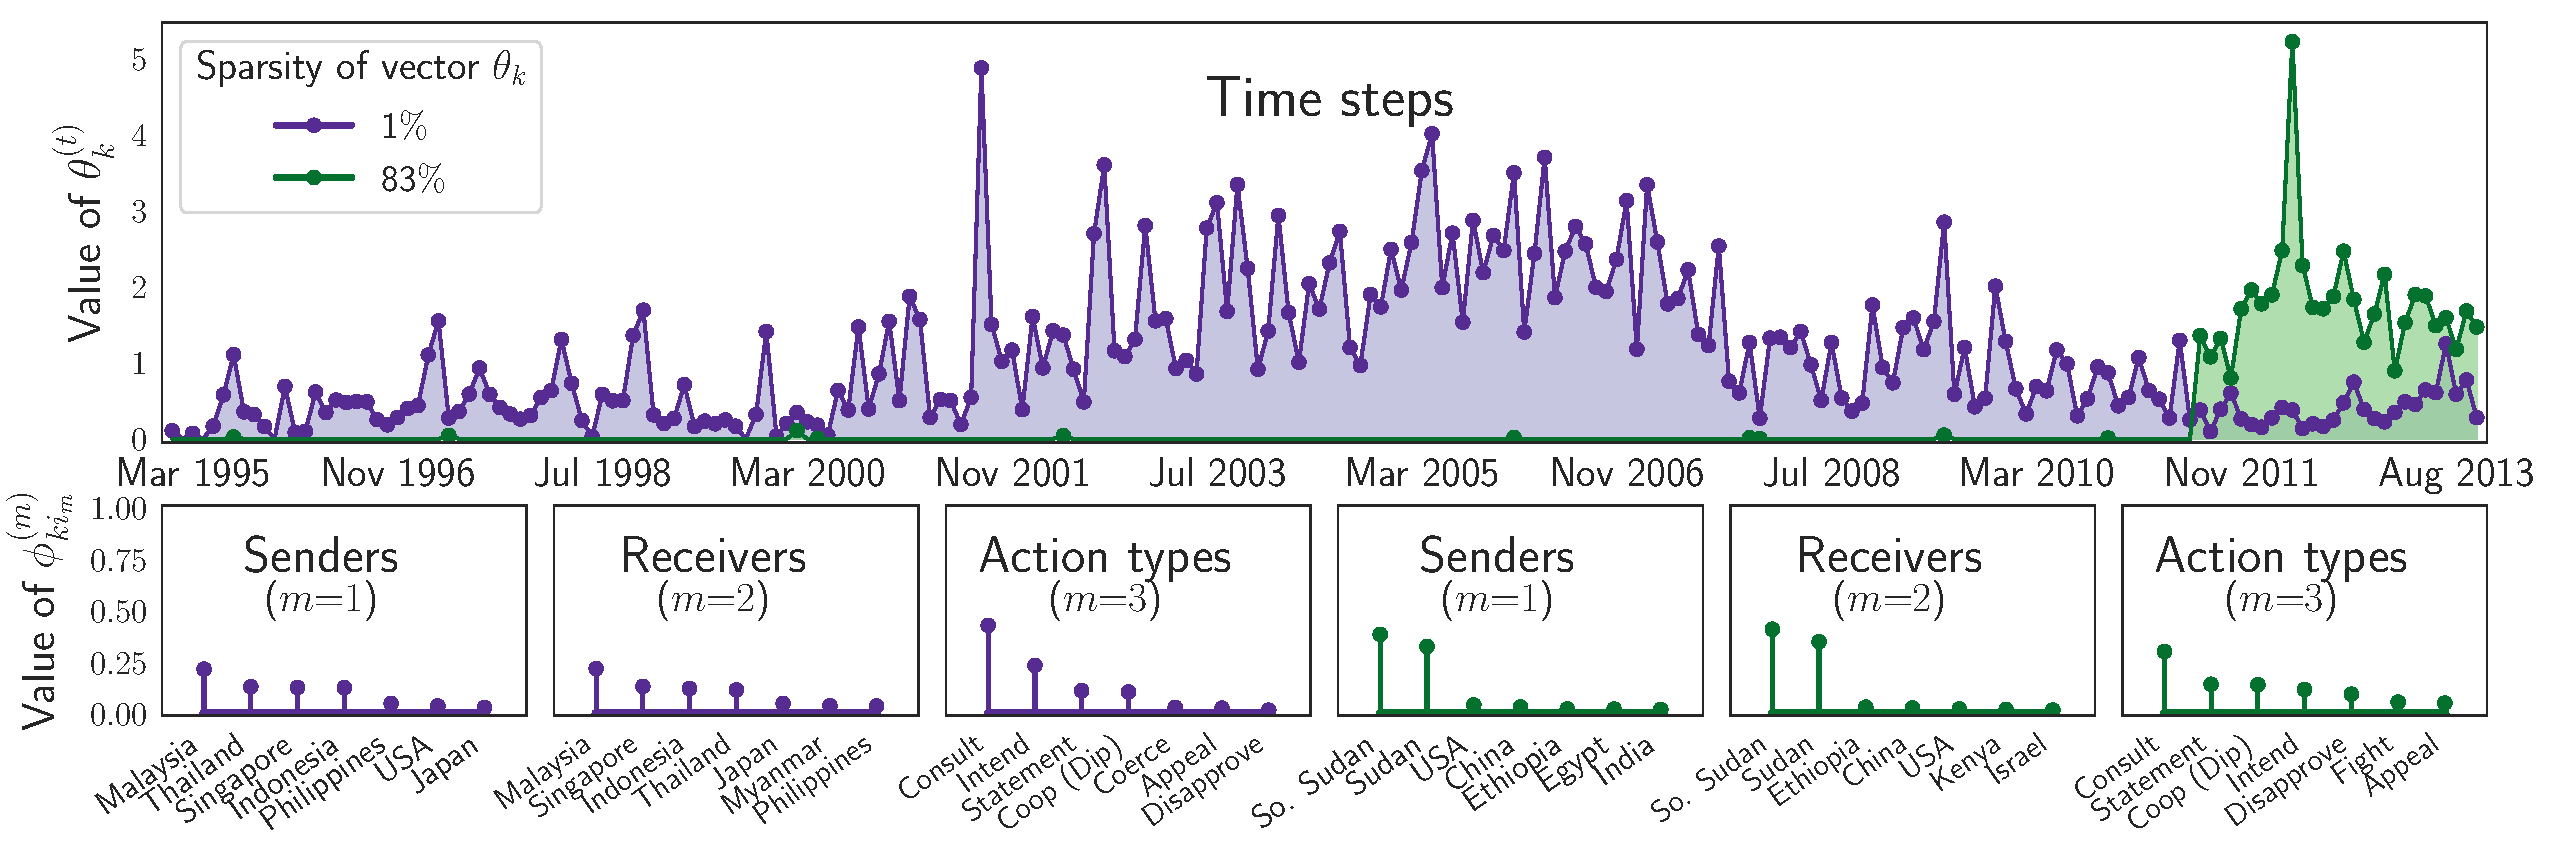
\includegraphics[width=\linewidth]{../../fig/components/icews/zero-ordering/double_plots/eps0-components72-0.pdf}
}
%
\hfill
\subfigure[\footnotesize Macaque motor cortex data]
{
\label{fig:macaque}
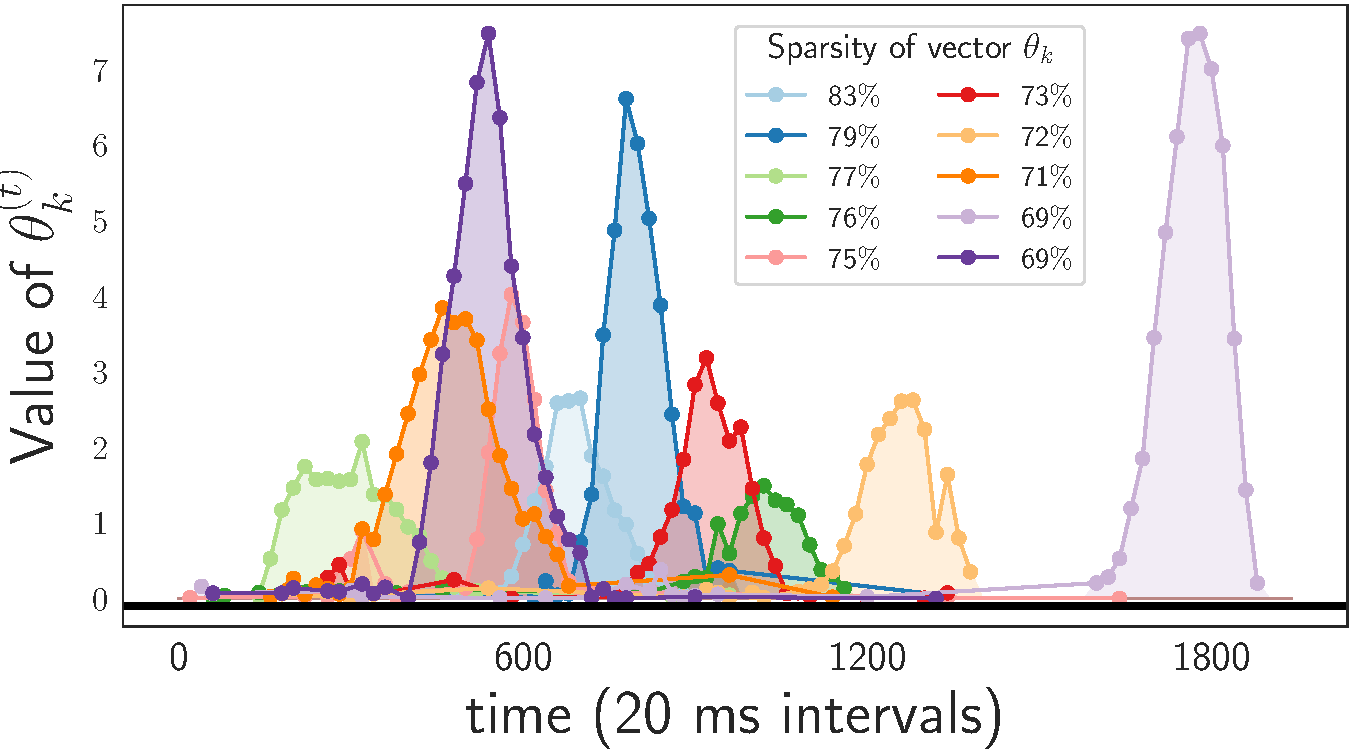
\includegraphics[width=0.49\linewidth]{../../results/tensors/monkeybrains/macaque_components_eps0.pdf}
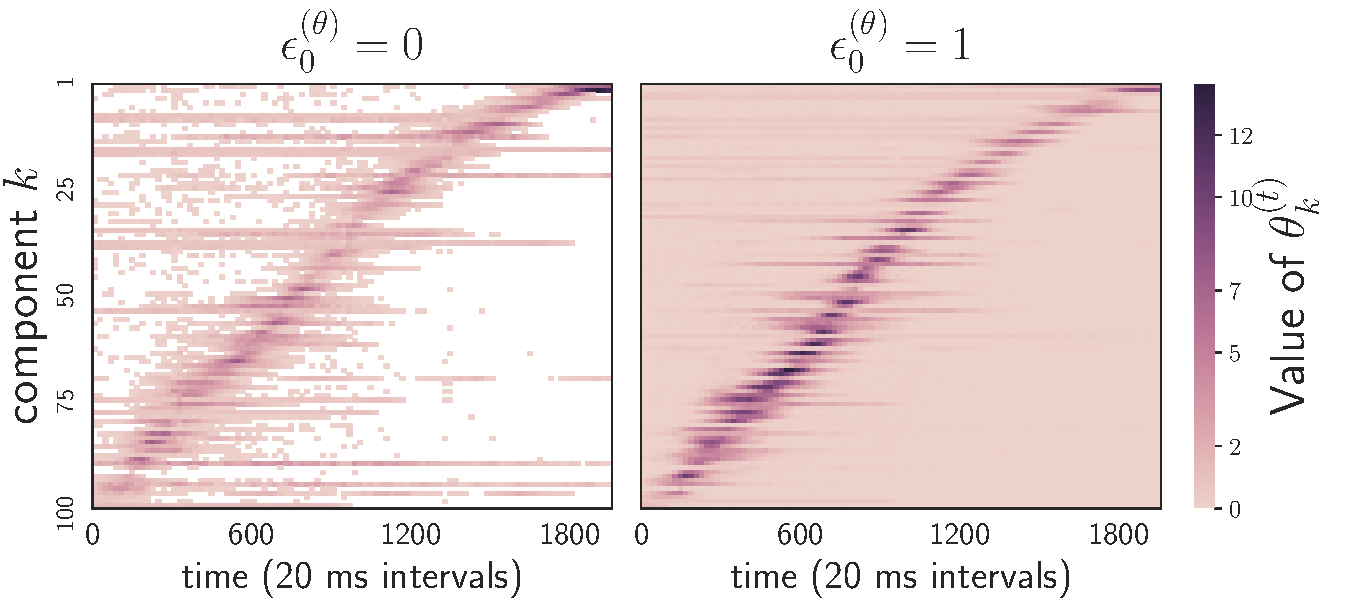
\includegraphics[width=0.49\linewidth]{../../results/tensors/monkeybrains/macaque_heat.pdf}
}
%
%
%\caption{\label{fig:exploratory} International event data (\cref{fig:sudan}) and macaque motor cortex data (\cref{fig:macaque}).}
\caption{\label{fig:exploratory} \Cref{fig:sudan} depicts two components inferred by a sparse variant of the PrGDS (i.e., $\epstheta \teq 0$) from the ICEWS data set. The blue component was also inferred by other models; the red component was not. The red component is specific to South Sudan, as revealed by visualizing the largest values of the sender and receiver factor vectors (bottom, red). South Sudan was not a country until July 2011. The gamma states (top, red) are thus sparse---i.e., $\thetakt \teq 0$ in 94\% of time steps (months) prior to July 2011 and in 83\% of the time steps overall. In contrast, the blue component represents Southeast Asian relations, which occur in all time steps. This variant of the PrGDS can infer both temporally persistent latent structures (e.g., blue), as well as bursty latent structures that are highly localized in time (e.g., red). \Cref{fig:macaque} depicts components inferred by the PrGDS from the macaque motor cortex data set. The components inferred by a sparse variant of the PrGDS (i.e., $\epstheta \teq 0$) are bursty and highly localized in time (left), suggesting that neurons may be tuned to specific periods of the trial. The $K \ttimes T$ gamma latent states for this variant of the PrGDS are sparse (middle, white cells correspond to $\thetakt\teq 0$). The components (rows) are sorted by the time step in which the largest $\thetakt$ occurred, so the banded structure indicates that each component is only active for a short duration. In contrast, the components inferred by the non-sparse variant of the PrGDS are active in all time steps (right).\looseness=-1}
\end{figure*}

\textbf{Discussion.} The PrGDS obtained the lowest perplexity in all
sixteen studies (see \cref{fig:empirical}) and a sparse variant of the
PrGDS (i.e., $\epstheta \teq 0$) obtained the lowest perplexity in
nine of the sixteen studies. We conjecture that the better performance
of the sparse variant can be explained by the form of the marginal
expectation of $\boldsymbol{\theta}^{\mathsmaller{(t)}}$ (see
\cref{eq:expectation}). When $\epstheta \!>\! 0$ this expectation
includes an additive term that grows as more time steps are
forecast. When $\epstheta \teq 0$, this term disappears and the
expectation matches that of the PGDS (see \cref{eq:pgds}). We also
performed a qualitative comparison of the latent structures inferred
by the different models and found that the sparse variant of the PrGDS
infers bursty latent structures that are highly localized in time. We
depict example components in \cref{fig:exploratory}.

%We describe in the Appendix how we aligned the inferred components across models, and provide examples of well-aligned components. We found several instances of bursty components inferred by the sparse PrGDS that could not be meaningfully aligned to any component inferred by the other models.~\looseness=-1

\section{Conclusion} We presented the Poisson-randomized gamma dynamical system (PrGDS), a tractable, expressive, and efficient model for sequentially observed count tensors. The PrGDS is based on a new modeling motif, an alternating chain of discrete Poisson and continuous gamma latent states that yields closed-form complete conditionals for all variables. We found that a sparse variant of the PrGDS, which allows the gamma latent states to take values of exactly zero, often obtains lower smoothing and forecasting perplexities than other models and infers latent structures that are highly localized in time.\looseness=-1


{\small
  \textbf{Acknowledgments} \;
  We thank Saurabh Vyas, Alex Williams, and Krishna Shenoy for kindly sharing the macaque monkey motor cortex data set and their preprocessing code.  AS was supported by TODO. SWL was supported by the Simons Collaboration on the Global Brain (SCGB 418011).  Mingyuan Zhou acknowledges the support of Award IIS-1812699 from the U.S. National Science Foundation.  DB was supported by TODO.}

% \begin{figure*}[t]
% \centering
% %
% \subfigure[\footnotesize Activation vectors $\boldsymbol{\theta}_k$ inferred by the sparse PrGDS.~\looseness=-1]
% {\label{fig:components}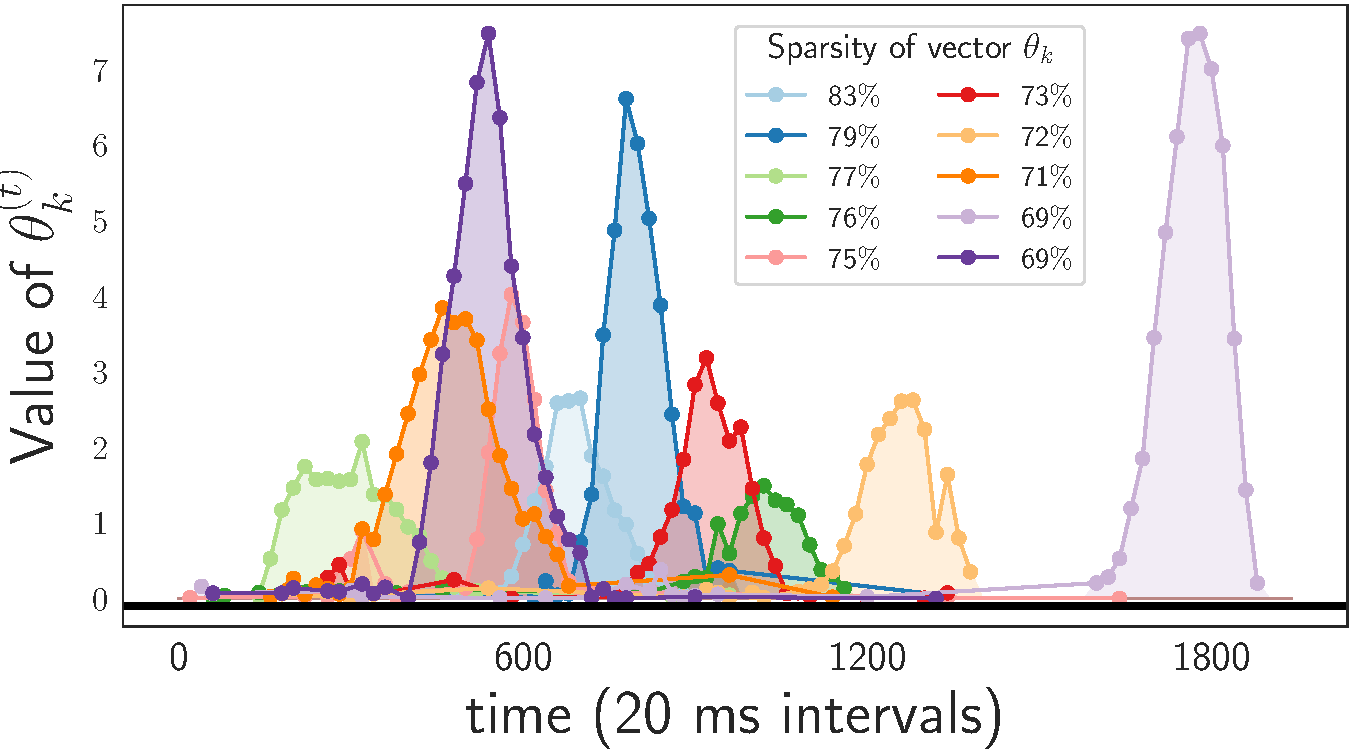
\includegraphics[width=0.49\linewidth]{../../results/tensors/monkeybrains/macaque_components_eps0.pdf}}\hfill
% %
% \subfigure[\footnotesize The full matrix $\Theta$ inferred by both PrGDS variants.~\looseness=-1]
% {\label{fig:heat}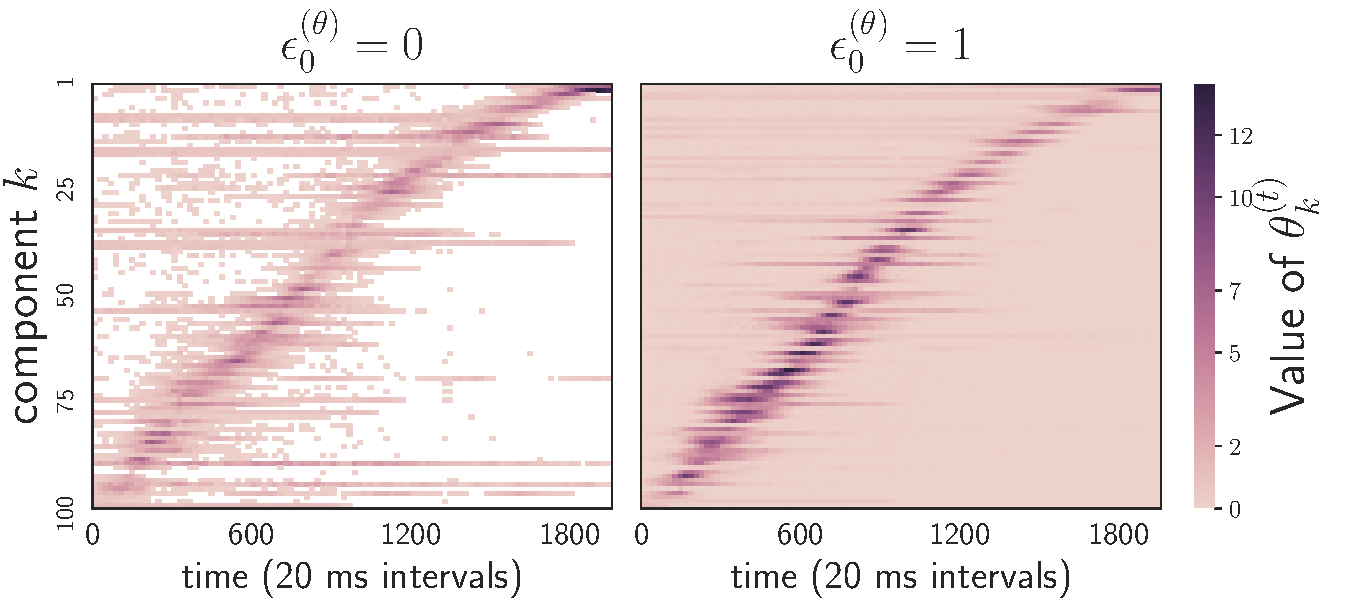
\includegraphics[width=0.49\linewidth]{../../results/tensors/monkeybrains/macaque_heat.pdf}} \vspace{-0.5em}
% %
% \caption{\label{fig:macaque} \footnotesize Two views of $\Theta$ inferred on Macaque tensor data. \cref{fig:heat} compares the $K \ttimes T$ state matrix inferred by the two PrGDS variants: $\epstheta \teq 0$ (sparse) vs. $\epstheta \teq 1$. The components $k$ are sorted according to which time step $t$ had the largest $\thetakt$---the visible banded structure suggests they both infer components that activate within specific short durations. White cells correspond to exact zeros $\thetakt\teq 0$---the PrGDS can represent truly sparse activation structure when $\epstheta \teq 0$. The $k^{\textrm{th}}$ row $\boldsymbol{\theta}_k$ is the $T$-length activation vector for component $k$---\cref{fig:components} provides an alternative visualization for ten of the sparssest activation vectors inferred by the sparse PrGDS. They collectively depict temporally localized and bursty neuronal spiking dynamics in accordance with neuroscientific accounts.~\looseness=-1}
% \end{figure*}


% \begin{figure*}[b]
% \centering
% 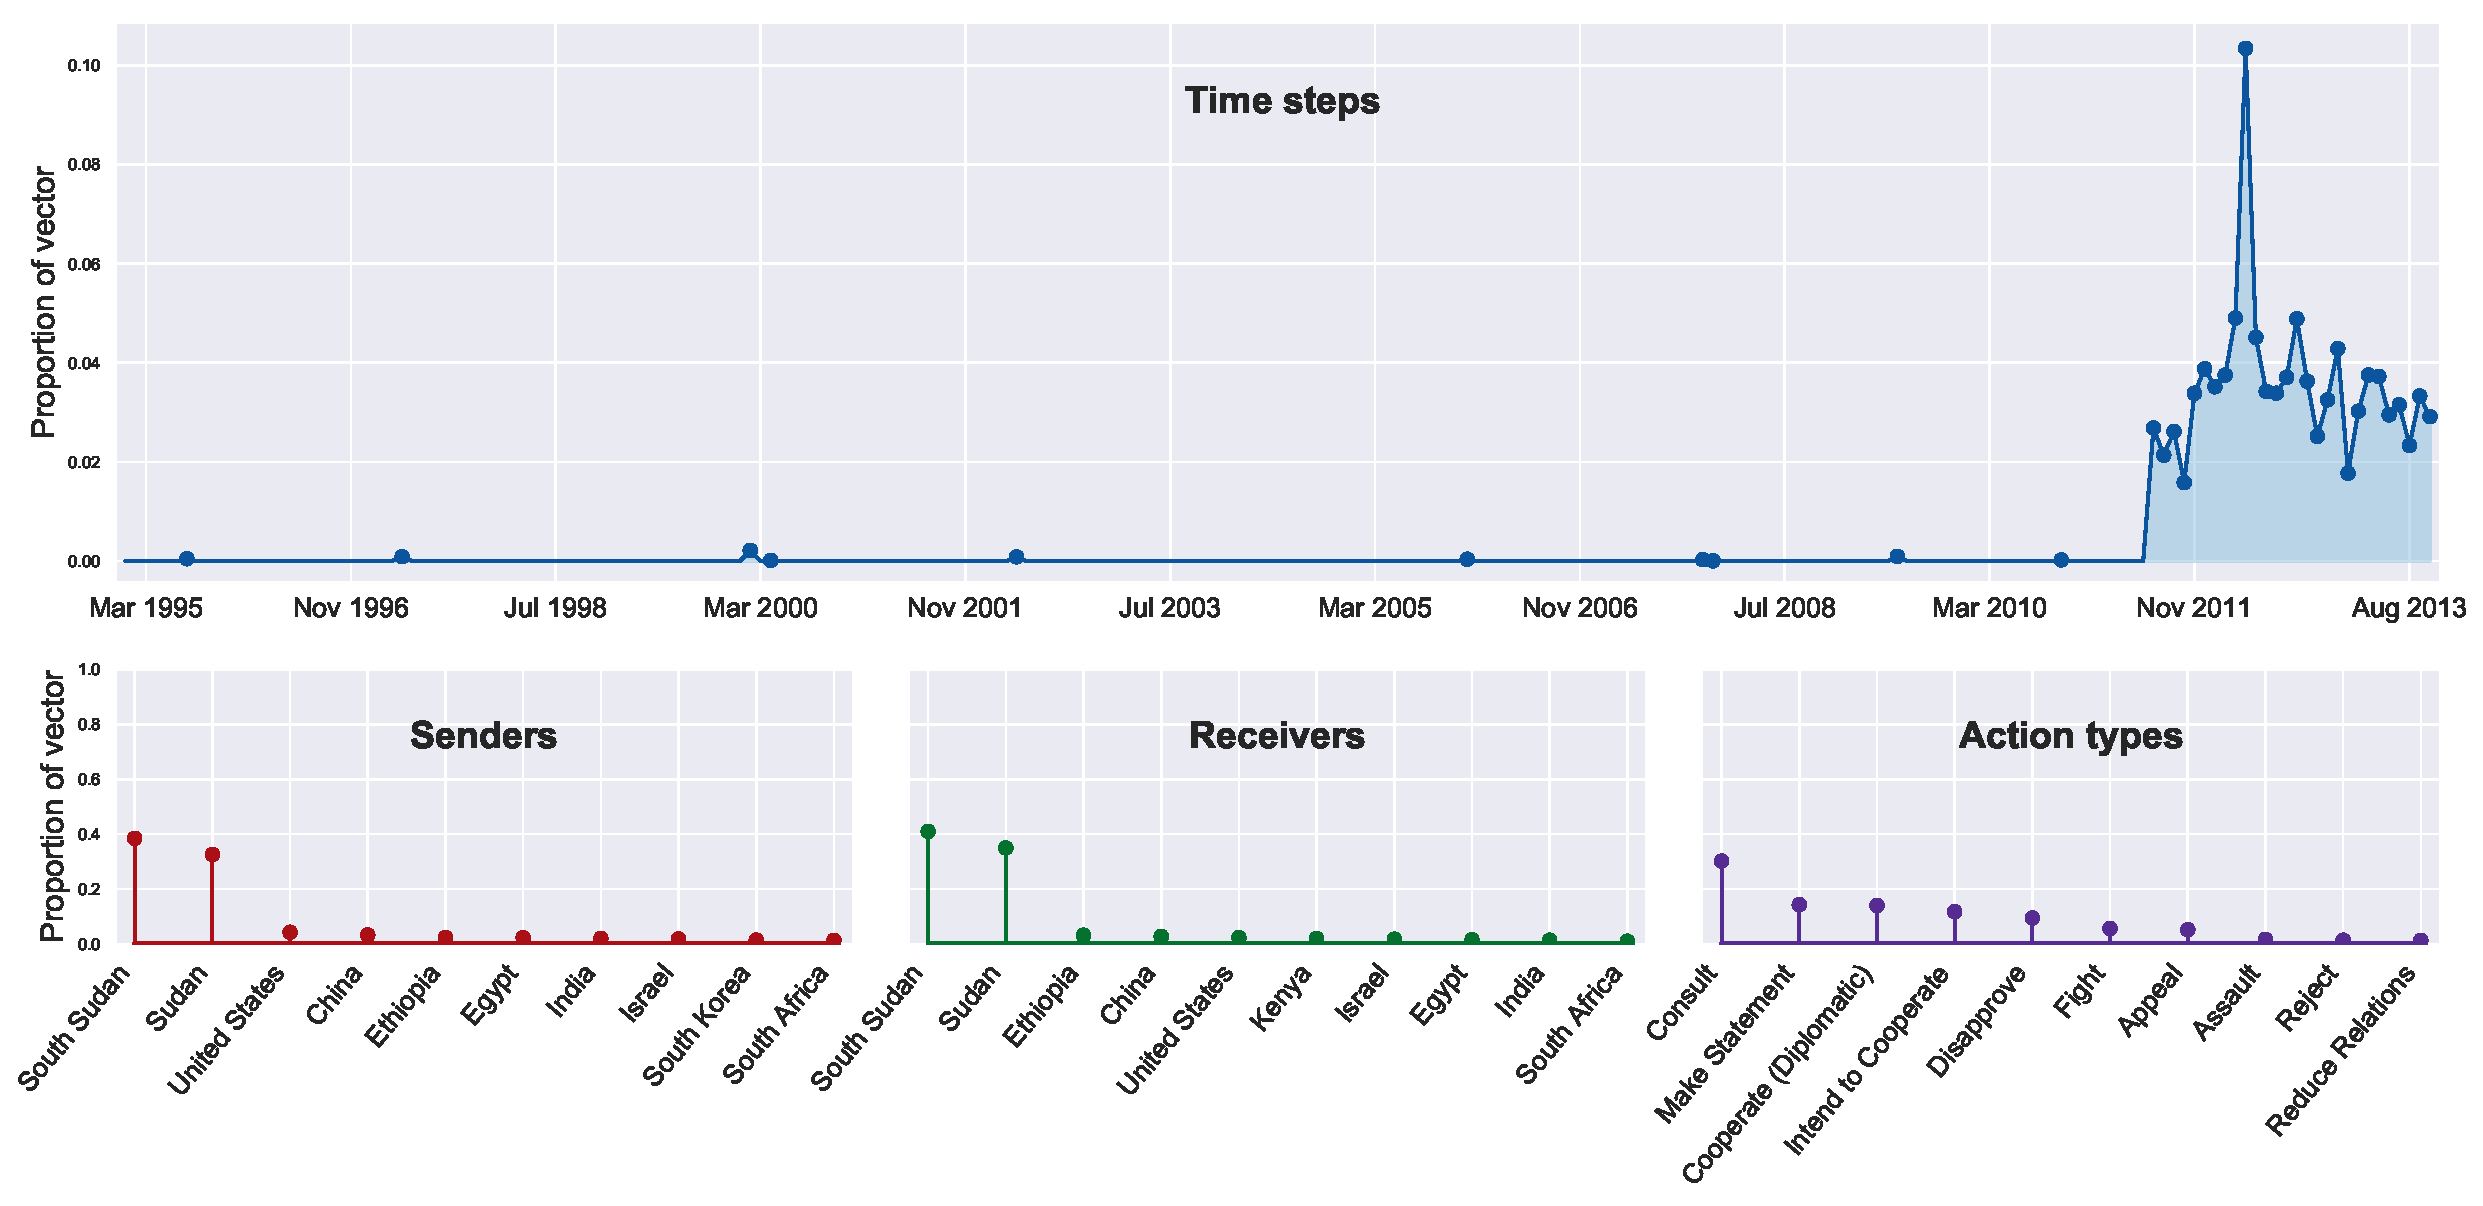
\includegraphics[width=\linewidth]{../../fig/components/icews/zero-ordering/new_plots/eps0-component-0.pdf}
% \caption{\footnotesize \label{fig:sudan} A variant of the PrGDS is capable of inferring true sparsity in its continuous latent states. When fit to dynamic tensor data of country--country interactions, this variant inferred the following component. \emph{Top row:} 94\% of the time steps (months) prior to July 2011 exhibit an inferred latent state value of exactly zero $\thetakt \teq 0$. \emph{Bottom left and middle:} This component mainly summarizes events involving South Sudan, a country that did not exist until July 2011. No other variant of the PrGDS found a component dedicated to South Sudan; we speculate that the sparse variant's unique inductive bias allows it surface patterns in the data that are highly localized in time.~\looseness=-1}
% \end{figure*}



% \section{Discussion}
% \begin{itemize}
% \item $\epstheta = 0$ is better as suggested by \cref{eq:expectation}.
% \item
% \end{itemize}
% \label{sec:conc}

\bibliographystyle{unsrtnat}
\bibliography{references}

\end{document}
